% ===========================================================================
% Raport de practică — Bunea Cosmin-Andrei
% Universitatea Transilvania din Brașov, FIESC, Calculatoare, anul III
% Stagiu Siemens SRL, 01.07.2026 – 30.09.2026
%
% Document de sine stătător. Compilare:  lualatex -> lualatex -> lualatex
% ===========================================================================
\documentclass[11pt,openany]{report}

% Compilat cu LuaLaTeX: literele romanesti cu virgula dedesubt au glife
% proprii in Latin Modern OpenType, nu sunt compuse din litera plus accent.
\usepackage{fontspec}
\setmainfont{Latin Modern Roman}[SmallCapsFont={Latin Modern Roman Caps}]
\setsansfont{Latin Modern Sans}
\setmonofont{Latin Modern Mono}
\usepackage[romanian]{babel}
\usepackage[a4paper,top=26mm,bottom=24mm,left=25mm,right=22mm,headheight=15pt]{geometry}

\usepackage{amsmath}
\usepackage{amssymb}
\usepackage{booktabs}
\usepackage{longtable}
\usepackage{tabularx}
\usepackage{array}
\usepackage{multirow}
\usepackage{enumitem}
\usepackage{xcolor}
\usepackage{fancyhdr}
\usepackage{titlesec}
\usepackage{caption}
\usepackage{float}
\usepackage{graphicx}
\usepackage{tikz}
\usepackage{tikz-timing}
\usetikzlibrary{arrows.meta,positioning,automata,calc,fit,backgrounds,
                shapes.geometric,shapes.misc,decorations.pathreplacing}
\usepackage[hidelinks,bookmarksnumbered]{hyperref}

% --- paletă ----------------------------------------------------------------
\definecolor{accent}{RGB}{0,72,110}
\definecolor{rulegrey}{RGB}{120,120,120}
\definecolor{boxbg}{RGB}{244,246,248}
\definecolor{rtlbg}{RGB}{238,242,236}
\definecolor{warnbg}{RGB}{252,246,232}

% --- antet / subsol --------------------------------------------------------
\pagestyle{fancy}
\fancyhf{}
\fancyhead[L]{\small\nouppercase{\leftmark}}
\fancyhead[R]{\small\thepage}
\fancyfoot[L]{\footnotesize Raport de practică --- Bunea Cosmin-Andrei}
\fancyfoot[R]{\footnotesize Siemens SRL, 2026}
\renewcommand{\headrulewidth}{0.4pt}
\renewcommand{\footrulewidth}{0.4pt}
\fancypagestyle{plain}{%
  \fancyhf{}%
  \fancyfoot[L]{\footnotesize Raport de practică --- Bunea Cosmin-Andrei}%
  \fancyfoot[R]{\footnotesize Siemens SRL, 2026}%
  \renewcommand{\headrulewidth}{0pt}%
  \renewcommand{\footrulewidth}{0.4pt}%
}

\titleformat{\chapter}[display]
  {\normalfont\Large\bfseries\color{accent}}
  {\chaptertitlename\ \thechapter}{6pt}{\LARGE}
\titlespacing*{\chapter}{0pt}{-14pt}{18pt}
\captionsetup{font=small,labelfont={bf,color=accent},skip=5pt}

% --- macrouri --------------------------------------------------------------
\newcommand{\sig}[1]{\texttt{#1}}
\newcommand{\mdl}[1]{\texttt{#1}}
\newcommand{\reg}[1]{\texttt{#1}}

\newenvironment{nota}
  {\par\vspace{4pt}\noindent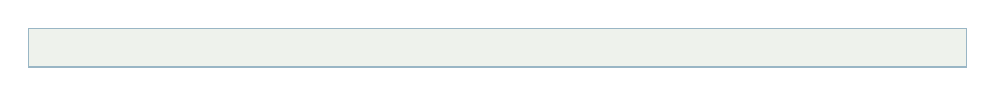
\begin{tikzpicture}\node[draw=accent!40,fill=rtlbg,line width=0.4pt,
    inner sep=7pt,text width=\dimexpr\linewidth-20pt\relax,align=justify,font=\small]\bgroup}
  {\egroup;\end{tikzpicture}\par\vspace{4pt}}

\newenvironment{atentie}
  {\par\vspace{4pt}\noindent
\begin{tikzpicture}\node[draw=orange!60,fill=warnbg,line width=0.4pt,
    inner sep=7pt,text width=\dimexpr\linewidth-20pt\relax,align=justify,font=\small]\bgroup}
  {\egroup;\end{tikzpicture}\par\vspace{4pt}}

\newcolumntype{L}[1]{>{\raggedright\arraybackslash}p{#1}}
\newcolumntype{C}[1]{>{\centering\arraybackslash}p{#1}}

\tikzset{
  blk/.style={draw=accent,fill=white,rounded corners=1.5pt,align=center,
              inner sep=5pt,font=\small,minimum height=9mm},
  blkf/.style={blk,fill=boxbg},
  regbox/.style={draw=rulegrey,fill=boxbg,align=center,inner sep=4pt,font=\footnotesize},
  flow/.style={-{Stealth[length=2.4mm]},thick,draw=accent},
  flowd/.style={flow,dashed},
  lbl/.style={font=\scriptsize,inner sep=1.5pt,fill=white},
  st/.style={draw=accent,circle,fill=white,minimum size=13mm,font=\small,inner sep=1pt,align=center},
  stb/.style={draw=accent,fill=white,rounded corners=2pt,align=center,
              font=\small,inner xsep=5pt,inner ysep=4pt,
              minimum height=8mm,minimum width=19mm},
  stbi/.style={stb,double,double distance=0.6pt},
}

\begin{document}

% ===========================================================================
% Pagina de titlu
% ===========================================================================
\begin{titlepage}
\centering


\includegraphics[width=62mm]{assets/Logo-UT-NEGRU-RO.pdf}\\[9mm]

{\large\scshape Universitatea Transilvania din Brașov}\\[2mm]
{\large Facultatea de Inginerie Electrică și Știința Calculatoarelor}\\[1.5mm]
{\normalsize Programul de studii \textbf{Calculatoare} --- Anul III}\\[13mm]

{\color{accent}\rule{\linewidth}{1.2pt}}\\[5mm]
{\Huge\bfseries RAPORT DE PRACTICĂ}\\[6mm]
{\LARGE Proiectarea și verificarea unui\\[2mm] System-on-Chip RV32I}\\[5mm]
{\large\itshape Procesor, controler de întreruperi și integrarea\\[1mm]
 pe magistrală AXI4 a unui sistem complet}\\[5mm]
{\color{accent}\rule{\linewidth}{1.2pt}}

\vfill

\begin{tabular}{@{}L{0.30\linewidth}L{0.52\linewidth}@{}}
\toprule
Student & \textbf{Bunea Cosmin-Andrei} \\
\addlinespace
Instituția gazdă & Siemens SRL --- Electronic Design Romania\newline
                   AFI Park 1, Bd.\ 15 Noiembrie nr.\ 78, Brașov \\
\addlinespace
Coordonator din partea\newline instituției gazdă
                 & Dávid Borzási \\
\addlinespace
Director de departament & Ș.l.\ dr.\ ing.\ STANCA Aurel-Cornel \\
\addlinespace
Perioada stagiului & 01.07.2026 --- 30.09.2026 \\
\addlinespace
Anul universitar & 2025/2026 \\
\bottomrule
\end{tabular}

\vspace{14mm}
\end{titlepage}

% ===========================================================================
\pagenumbering{roman}
\setcounter{page}{2}

\chapter*{Despre acest raport}
\addcontentsline{toc}{chapter}{Despre acest raport}
\markboth{Despre acest raport}{}

Raportul descrie ce am proiectat, ce am integrat și ce am verificat până acum în
stagiul de la Siemens, în programul \emph{Digital IC Design \& Advanced
Verification}. Stagiul este în curs și se încheie la 30 septembrie 2026.

Protocolul AXI4, în măsura în care acest sistem îl folosește, și instrumentele de
lucru sunt în Anexa~\ref{ch:tehnologii}.

Cifrele din capitolul de verificare sunt citite din jurnalul regresiei rulate pe
versiunea curentă a proiectului.

\tableofcontents
\listoffigures

\cleardoublepage
\pagenumbering{arabic}
\setcounter{page}{1}

% ===========================================================================
\chapter{Contextul stagiului}
\label{ch:context}

\section{Instituția gazdă}

Am efectuat stagiul de practică la \textbf{Siemens SRL}, în departamentul
\emph{Electronic Design Romania}, cu sediul în AFI Park 1, Bulevardul 15
Noiembrie nr.~78, Brașov. Coordonator din partea instituției gazdă a fost domnul
\textbf{Dávid Borzási}.

Siemens face parte dintr-un grup tehnologic prezent global, cu activități în
industrie, infrastructură, mobilitate și sănătate. Divizia relevantă pentru
stagiu este Siemens EDA, care dezvoltă instrumente de proiectare și verificare
pentru circuite ASIC, FPGA și SoC: simulare și verificare funcțională sau
formală, verificare fizică și a fiabilității, simulare analogică, precum și
soluții embedded construite pe arhitectura RISC-V, destinate aplicațiilor auto,
industriale, aerospațiale și medicale. Stagiul s-a desfășurat exact pe acest
teren --- proiectare RTL și verificare, cu instrumentele și convențiile folosite
industrial.

\section{Obiectivul stagiului}

Tema stagiului --- \emph{Digital IC Design \& Advanced Verification} --- a fost
proiectarea de la zero a unui System-on-Chip funcțional și verificarea lui.
Punctul de plecare, stabilit în ședința de deschidere din 1 iulie 2026, a fost
modelul clasic al unui SoC: un nucleu de calcul, o magistrală care îl leagă de
periferice și memorii, și un motor de transfer care mută date în fundal, fără să
consume timp de procesor.

Fluxul de date țintă a fost enunțat de la început în cinci pași, iar el a rămas
criteriul de acceptare al întregului proiect:

\begin{enumerate}[itemsep=1pt,topsep=3pt]
\item procesorul configurează motorul DMA prin registre, peste AXI4-Lite;
\item DMA-ul citește și scrie date folosind propria interfață de master AXI4;
\item memoria SRAM dual-port servește ca tampon partajat între procesor și DMA;
\item DMA-ul semnalează terminarea transferului printr-o întrerupere;
\item procesorul prelucrează datele noi.
\end{enumerate}

Obiectivul nu a fost, așadar, un bloc izolat care trece un testbench, ci un
sistem în care software rulând pe procesorul propriu programează un periferic
propriu, adoarme, este trezit de o întrerupere reală și verifică rezultatul.
Acest scenariu rulează astăzi ca test de sistem și este descris în
Capitolul~\ref{ch:verificare}.

\section{Echipa și repartizarea temelor}
\label{sec:echipa}

Am lucrat în echipă de trei stagiari. Împărțirea a fost făcută pe blocuri, cu un
document de cerințe separat pentru fiecare, astfel încât cele trei blocuri să
poată fi dezvoltate în paralel și integrate la sfârșit.

\begin{table}[H]
\centering
\caption{Repartizarea temelor și responsabilitatea fiecărui bloc}
\label{tab:echipa}
\small
\begin{tabular}{@{}lL{0.24\linewidth}L{0.42\linewidth}@{}}
\toprule
\textbf{Coleg} & \textbf{Bloc} & \textbf{Conținut} \\
\midrule
Gabriel & Memorie SRAM dual-port &
  Două porturi AXI4-Lite independente, 1~KB, detecție și arbitrare de
  coliziuni, registre de control și de monitorizare a lățimii de bandă. \\
\addlinespace
Andrei & Motor DMA multi-canal &
  Patru canale independente, scatter-gather pe lanțuri de descriptori, master
  AXI4-Full cu rafale, arbitru de prioritate, limitare de bandă per canal. \\
\addlinespace
\textbf{Bunea Cosmin-Andrei} & \textbf{Procesor RV32I, controler de
  întreruperi, temporizator} &
  Pipeline pe trei stagii, două porturi master AXI4-Lite, controler de
  întreruperi cu 16 surse hardware și 16 software, temporizator de sistem pe
  64 de biți. \\
\bottomrule
\end{tabular}
\end{table}

Pe lângă blocul propriu mi-am asumat și \textbf{integrarea celor trei
blocuri într-un SoC func\-țio\-nal}. Aceasta a însemnat scrierea magistralei care le leagă
--- decodor de adrese, arbitru, punte de protocol, memorii AXI4-Lite ---, a
nivelului de vârf al sistemului și a verificării la nivel de sistem. Este partea
descrisă în Capitolul~\ref{ch:integrare} și, ca volum de muncă, a fost
comparabilă cu proiectarea procesorului.

\begin{nota}
\textbf{De ce a contat separarea pe ramuri.} Fiecare bloc s-a dezvoltat pe ramura
lui, cu testbench-urile lui, fără să depindă de starea celorlalte două. La
integrare, cele trei ramuri au fost aduse împreună fără să fie rescrise: nicio
ramură de bloc nu a fost rebazată sau suprascrisă. Consecința practică este că
fiecare coleg a putut continua să lucreze la blocul lui în timp ce integrarea era
în curs, iar o greșeală de integrare nu putea să corupă munca nimănui.
\end{nota}

\section{Interfața dintre blocuri, stabilită de la început}

Cele trei blocuri nu s-ar fi putut integra dacă nu ne-am fi înțeles din prima
săptămână asupra a trei lucruri. Odată fixate, nu s-au mai schimbat:

\begin{itemize}[itemsep=4pt,topsep=3pt]
\item \textbf{Un singur protocol de magistrală.} Toate porturile de tip slave
      sunt AXI4-Lite pe 32 de biți. Singura excepție admisă a fost portul de
      master al DMA-ului, care este AXI4-Full, pentru că un motor de transfer
      își pierde rostul dacă nu poate emite rafale. Această excepție este
      motivul pentru care sistemul are nevoie de o punte de protocol, subiectul
      Secțiunii~\ref{sec:punte}.
\item \textbf{Un singur domeniu de ceas și un singur reset}, asincron și activ
      pe \texttt{0}. Nicio traversare între domenii de ceas nu apare în sistem,
      ceea ce elimină o clasă întreagă de defecte care oricum nu ar fi putut fi
      verificată în timpul disponibil.
\item \textbf{Întreruperile trec toate prin controlerul de întreruperi.} Niciun
      periferic nu se leagă direct la procesor; fiecare își ridică linia
      proprie, iar controlerul decide care ajunge la nucleu și în ce ordine.
\end{itemize}

\section{Etapele lucrării}

Stagiul se desfășoară între 1 iulie și 30 septembrie 2026, în regim hibrid: lucru
individual pe parcursul săptămânii și o întâlnire săptămânală cu coordonatorul,
la sediu. Întâlnirea are de fiecare dată aceeași structură --- ce am făcut de la
ultima discuție, cum arată progresul față de ce era planificat, ce urmează, și
feedback pe deciziile luate între timp. Acest ritm este și motivul pentru care
etapele de mai jos se citesc ca o secvență și nu ca o listă de sarcini paralele:
fiecare a fost discutată și acceptată înainte să înceapă următoarea.

Etapele parcurse până la data acestui raport sunt, în ordine:

\begin{table}[H]
\centering
\caption{Etapele lucrării proprii, în ordine cronologică}
\label{tab:etape}
\small
\begin{tabular}{@{}L{0.20\linewidth}L{0.70\linewidth}@{}}
\toprule
\textbf{Perioadă} & \textbf{Ce am făcut} \\
\midrule
Iulie,\newline prima jumătate &
  Arhitectura procesorului: datapath modular, registre între stagii, decodor,
  generator de imediate, ALU, logica de hazarduri, predictor de branch, unitatea
  load/store și cele două interfețe AXI4-Lite. \\
\addlinespace
Iulie,\newline a doua jumătate &
  Controlerul de întreruperi și temporizatorul, registrele de control și stare,
  instrucțiunea de așteptare \sig{WFI}, stiva adreselor de retur, contoarele
  hardware de performanță. Prima infrastructură de verificare: testbench-uri
  auto-verificatoare, monitoare de protocol, aserțiuni, integrare continuă. \\
\addlinespace
August &
  Reproiectarea controlerului de întreruperi pentru 16 surse hardware și 16
  software, cu benzi de prioritate, preempție și nesting. Eliminarea
  avertismentelor de compilare, reset determinist pe fiecare bistabil,
  extinderea regresiei cu teste de bloc separate. Redactarea documentației
  tehnice. \\
\addlinespace
Sfârșit de august\newline --- 1 septembrie &
  Integrarea: organizarea depozitului pe blocuri, magistrala AXI4-Lite, puntea
  AXI4-Full $\rightarrow$ AXI4-Lite, nivelul de vârf, testele de sistem și de
  stres, revizuirea adversarială a propriei lucrări și fixarea prin teste a
  proprietăților pe care le-a stabilit. \\
\bottomrule
\end{tabular}
\end{table}

% ===========================================================================
\chapter{Arhitectura sistemului}
\label{ch:arhitectura}

\section{Calea de date}

Sistemul are trei masteri --- portul de instrucțiuni al procesorului, portul lui
de date, și portul de master al DMA-ului --- și șase slave-uri. Între ei stă o
magistrală pe care am scris-o eu în întregime: trei decodoare de adrese, un
arbitru, o punte de protocol și două memorii, adică șapte instanțe ale celor
patru module descrise în Capitolul~\ref{ch:integrare}.

\begin{figure}[H]
\centering
\resizebox{\linewidth}{!}{%
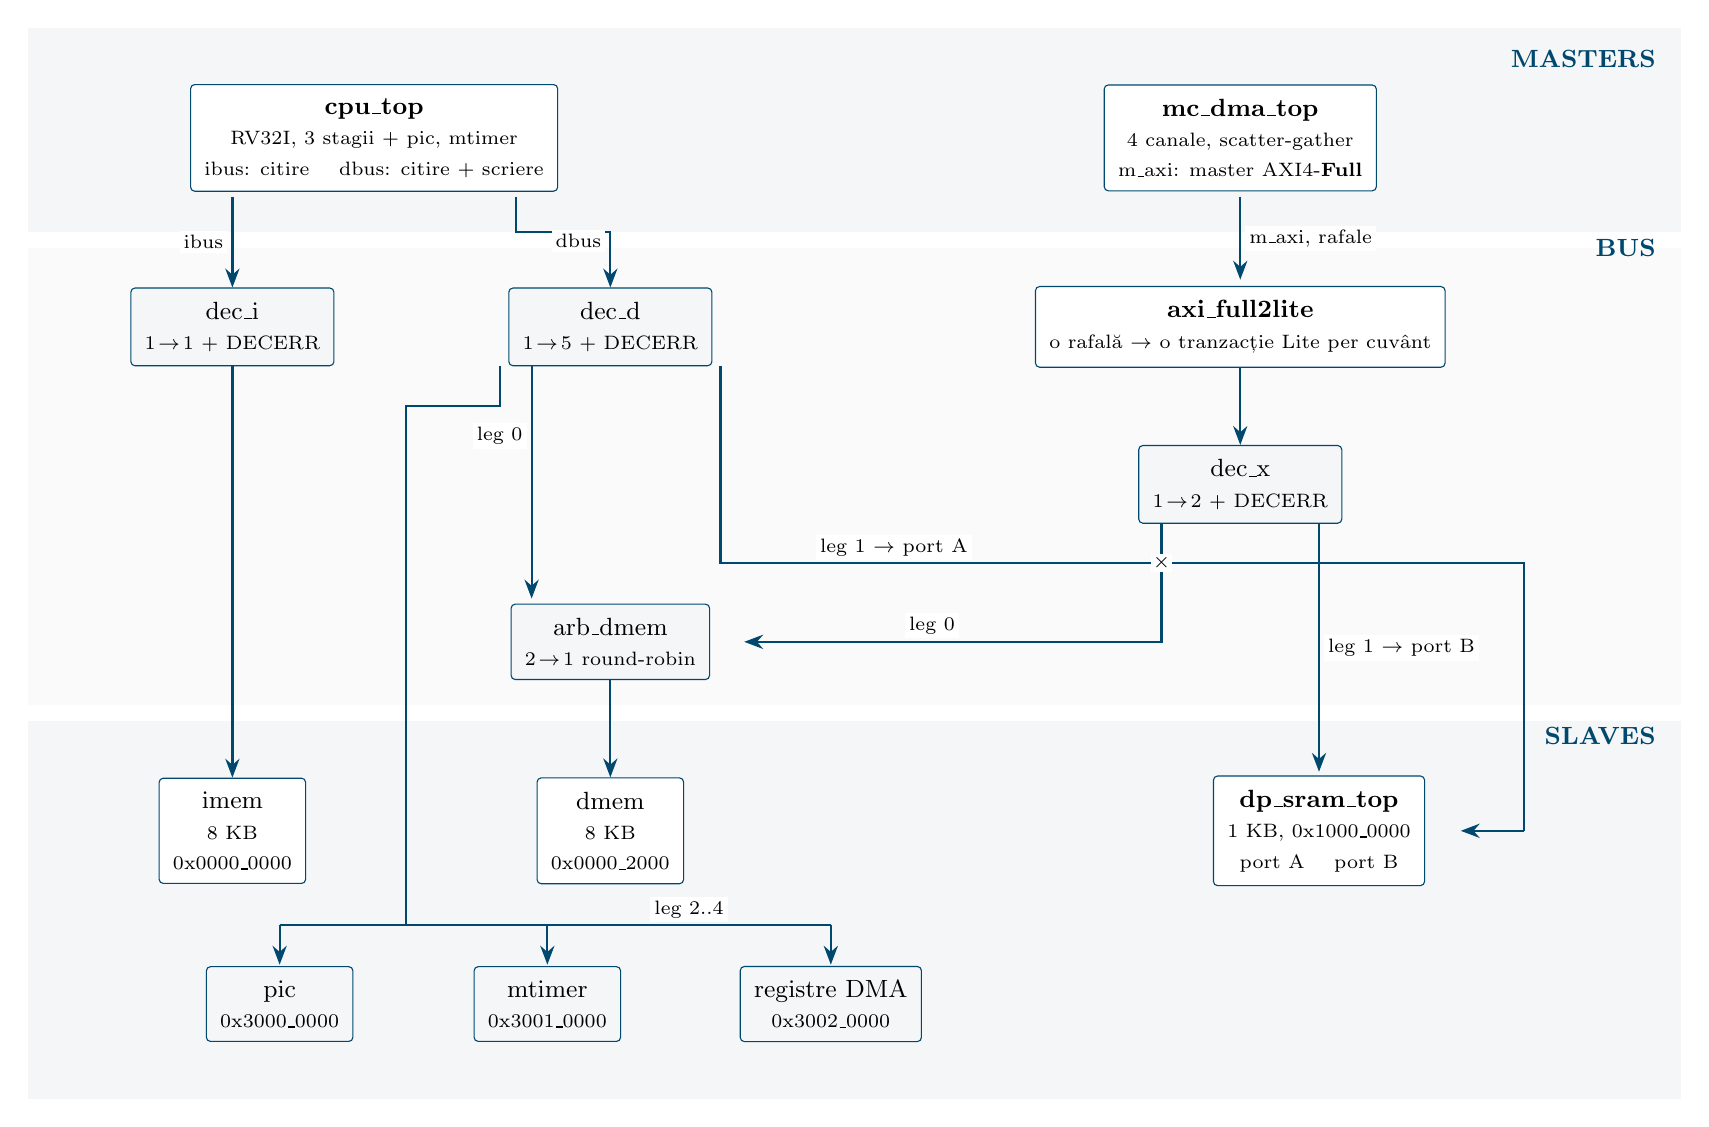
\begin{tikzpicture}[x=1mm,y=1mm,font=\small]

  % --- benzi de fundal ----------------------------------------------------
  \begin{scope}[on background layer]
    \fill[boxbg]    (-14,86)  rectangle (196,112);
    \fill[boxbg!50] (-14,26)  rectangle (196,84);
    \fill[boxbg]    (-14,-24) rectangle (196,24);
  \end{scope}
  \node[font=\small\bfseries,color=accent,anchor=east] at (194,108) {MASTERS};
  \node[font=\small\bfseries,color=accent,anchor=east] at (194,84)  {BUS};
  \node[font=\small\bfseries,color=accent,anchor=east] at (194,22)  {SLAVES};

  % --- masteri ------------------------------------------------------------
  \node[blk,minimum width=56,minimum height=15] (cpu) at (30,98)
        {\textbf{cpu\_top}\\\scriptsize RV32I, 3 stagii $+$ pic, mtimer
         \\\scriptsize ibus: citire \quad dbus: citire $+$ scriere};
  \node[blk,minimum width=48,minimum height=15] (dma) at (140,98)
        {\textbf{mc\_dma\_top}\\\scriptsize 4 canale, scatter-gather
         \\\scriptsize m\_axi: master AXI4-\textbf{Full}};

  % --- magistrală ---------------------------------------------------------
  \node[blkf,minimum width=26,minimum height=10] (deci) at (12,74)
        {dec\_i\\\scriptsize $1\!\to\!1$ + DECERR};
  \node[blkf,minimum width=30,minimum height=10] (decd) at (60,74)
        {dec\_d\\\scriptsize $1\!\to\!5$ + DECERR};
  \node[blk,minimum width=46,minimum height=12]  (brg)  at (140,74)
        {\textbf{axi\_full2lite}\\\scriptsize o rafală $\to$ o tranzacție Lite per cuvânt};
  \node[blkf,minimum width=32,minimum height=10] (decx) at (140,54)
        {dec\_x\\\scriptsize $1\!\to\!2$ + DECERR};
  \node[blkf,minimum width=34,minimum height=11] (arb)  at (60,34)
        {arb\_dmem\\\scriptsize $2\!\to\!1$ round-robin};

  % --- slave-uri ----------------------------------------------------------
  \node[blk,minimum width=28,minimum height=13] (imem) at (12,10)
        {imem\\\scriptsize 8 KB\\\scriptsize 0x0000\_0000};
  \node[blk,minimum width=28,minimum height=13] (dmem) at (60,10)
        {dmem\\\scriptsize 8 KB\\\scriptsize 0x0000\_2000};
  \node[blk,minimum width=36,minimum height=15] (sram) at (150,10)
        {\textbf{dp\_sram\_top}\\\scriptsize 1 KB, 0x1000\_0000
         \\\scriptsize port A \quad port B};

  \node[blkf,minimum width=26,minimum height=10] (pic) at (18,-12)
        {pic\\\scriptsize 0x3000\_0000};
  \node[blkf,minimum width=26,minimum height=10] (tmr) at (52,-12)
        {mtimer\\\scriptsize 0x3001\_0000};
  \node[blkf,minimum width=30,minimum height=10] (dmar) at (88,-12)
        {registre DMA\\\scriptsize 0x3002\_0000};

  % --- masteri -> decodoare ----------------------------------------------
  \draw[flow] (12,90.5) -- (12,79) node[lbl,midway,left=0.5mm]{ibus};
  \draw[flow] (48,90.5) -- (48,86) -- (60,86) -- (60,79) node[lbl,pos=0.15,left=0.5mm]{dbus};
  \draw[flow] (140,90.5) -- (140,80) node[lbl,midway,right=0.5mm]{m\_axi, rafale};
  \draw[flow] (brg.south) -- (decx.north);

  % --- dec_i -> imem ------------------------------------------------------
  \draw[flow] (deci.south) -- (imem.north);

  % --- dec_d: cele cinci ieșiri -------------------------------------------
  % leg 0: memoria de date, prin arbitru
  \draw[flow] (50,69) -- (50,39.5) node[lbl,pos=0.3,left=0.5mm]{leg 0};
  % legs 2..4: periferice, pe o magistrală orizontală sub arbitru
  \draw[flow,-] (46,69) -- (46,64) -- (34,64) -- (34,-2);
  \draw[thick,draw=accent] (18,-2) -- (88,-2);
  \foreach \x in {18,52,88} \draw[flow] (\x,-2) -- (\x,-7);
  \node[lbl,above=0.3mm] at (70,-2) {leg 2..4};
  % leg 1: portul A al memoriei duale, pe la marginea din dreapta
  \draw[flow,-] (74,69) -- (74,44) -- (176,44) -- (176,10);
  \draw[flow] (176,10) -- (168,10);
  \node[lbl,above=0.3mm] at (96,44) {leg 1 $\to$ port A};

  % --- dec_x: cele două ieșiri --------------------------------------------
  \draw[flow] (130,49) -- (130,34) -- (77,34) node[lbl,pos=0.55,above=0.3mm]{leg 0};
  \draw[flow] (150,49) -- (150,17.5) node[lbl,midway,right=0.5mm]{leg 1 $\to$ port B};

  % --- arbitru -> memoria de date -----------------------------------------
  \draw[flow] (arb.south) -- (dmem.north);

  % singura încrucișare din figură, în spațiu liber
  \node[lbl,fill=white,inner sep=0.6pt] at (130,44) {$\times$};

\end{tikzpicture}}
\caption{Calea de date a sistemului. Cutiile din banda mijlocie sunt blocurile
pe care le-am scris pentru integrare; cele din banda de sus și de jos sunt
blocurile de proiectare, ale mele și ale colegilor. Cele două trasee care se
încrucișează --- portul A al memoriei duale, alimentat dinspre stânga, și
prima ieșire a decodorului DMA, care merge spre dreapta --- nu pot fi desenate
fără o încrucișare; ea este marcată cu $\times$ și se află în spațiu liber.}
\label{fig:soc}
\end{figure}

Două trasee prin magistrală, urmărite de la un capăt la altul:

\begin{itemize}[itemsep=3pt,topsep=3pt]
\item \textbf{O încărcare din memoria duală, făcută de procesor.} Portul de date
      intră în \mdl{dec\_d}, iese pe ieșirea~1 și ajunge direct la portul~A al
      memoriei. Nu există arbitru pe acest traseu: portul~A îi aparține
      procesorului în întregime.
\item \textbf{DMA-ul mutând 32 de octeți din memoria de date.} Portul de master
      emite o singură rafală \sig{INCR} de opt cuvinte. Puntea o desface în opt
      tranzacții AXI4-Lite separate, care intră în \mdl{dec\_x}, ies pe
      ieșirea~0 și ajung la arbitru, unde fiecare se așază la coadă în spatele
      cererilor procesorului.
\end{itemize}

\section{Harta de adrese}

Harta este definită într-un singur loc, iar decodoarele o primesc ca parametru.
Trei proprietăți ale ei sunt decizii, nu valori implicite, și fiecare are un
test dedicat care cade dacă proprietatea se pierde.

\begin{table}[H]
\centering
\caption{Harta de adrese și accesibilitatea. O celulă goală înseamnă că masterul
respectiv nu are nicio cale către acel slave; un acces acolo primește
\sig{DECERR}.}
\label{tab:addrmap}
\small
\begin{tabular}{@{}llrccc@{}}
\toprule
\textbf{Slave} & \textbf{Bază} & \textbf{Dim.} &
\textbf{ibus} & \textbf{dbus} & \textbf{DMA} \\
\midrule
imem      & \texttt{0x0000\_0000} & 8 KB   & \checkmark & --- & --- \\
dmem      & \texttt{0x0000\_2000} & 8 KB   & --- & \checkmark & \checkmark \\
dp\_sram  & \texttt{0x1000\_0000} & 1 KB   & --- & \checkmark (A) & \checkmark (B) \\
pic       & \texttt{0x3000\_0000} & 256 B  & --- & \checkmark & --- \\
mtimer    & \texttt{0x3001\_0000} & 256 B  & --- & \checkmark & --- \\
registre DMA & \texttt{0x3002\_0000} & 256 B & --- & \checkmark & --- \\
\bottomrule
\end{tabular}
\end{table}

\paragraph{Fiecare fereastră are exact dimensiunea blocului ei.} Masca de
decodare a unei ferestre este exact mărimea blocului, nu mărimea intervalului
dintre blocuri. Perifericele sunt așezate din 64 în 64 de kiloocteți, dar
fiecare are o fereastră de numai 256 de octeți, fiindcă atât are banca lui de
registre. Dacă fereastra ar fi de 64~KB, adresa \texttt{0x3000\_0100} ar cădea
tot în controlerul de întreruperi și ar ateriza pe primul lui registru,
răspunzând \sig{OKAY} --- adică exact eșecul pe care decodorul există ca să-l
prevină. Cu fereastra de 256 de octeți, aceeași adresă nu nimerește nicio
fereastră și primește \sig{DECERR}.

\paragraph{Accesibilitatea nu este uniformă, și asta este intenționat.} Portul
de instrucțiuni ajunge numai la memoria de instrucțiuni, deci un contor de
program scăpat de sub control primește o eroare de decodare în loc să execute
registrele unui periferic. Portul de date ajunge peste tot în afară de memoria
de instrucțiuni, deci nu există cale prin care programul să-și rescrie propriul
cod. DMA-ul ajunge numai la memoria de date și la memoria duală, deci un
descriptor greșit nu poate reprograma controlerul de întreruperi.

\paragraph{Memoria duală este văzută la aceeași adresă din ambele părți.}
Procesorul o atinge pe portul~A, DMA-ul pe portul~B, ambii la
\texttt{0x1000\_0000}. Acesta este lucrul care ține detectorul de coliziuni al
blocului viu în sistemul asamblat: dacă cei doi masteri ar vedea memoria la
adrese diferite, nu s-ar putea ciocni niciodată pe același cuvânt.

\section{Harta întreruperilor}

Niciun periferic nu se leagă direct la procesor. Fiecare își ridică linia
proprie către controlerul de întreruperi, iar acesta oferă nucleului o singură
cerere, pe cea mai urgentă.

\begin{figure}[H]
\centering
\resizebox{\linewidth}{!}{%
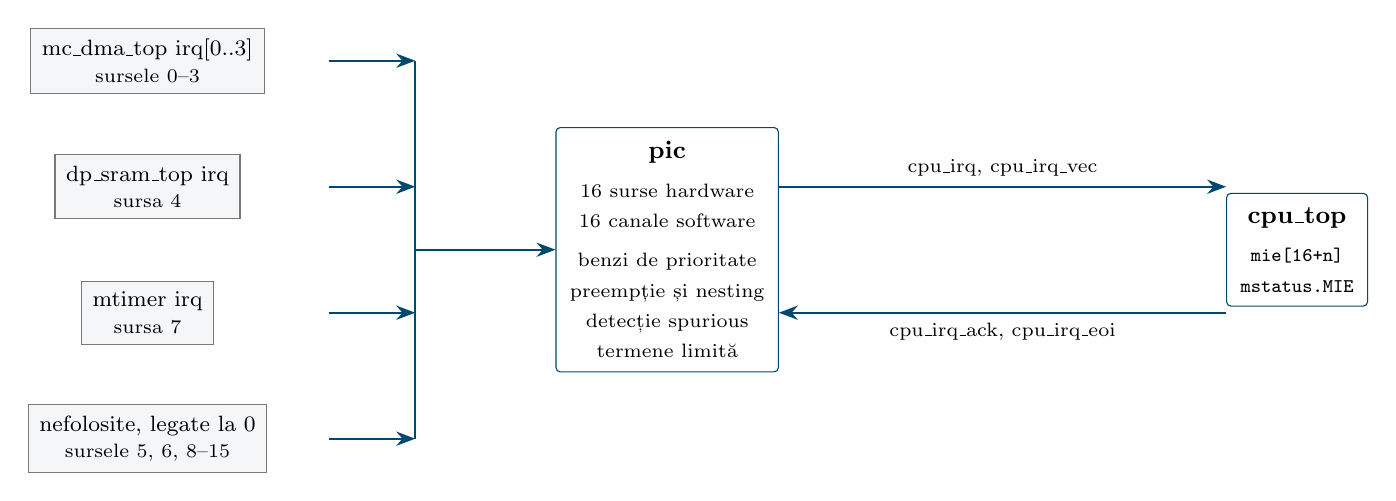
\begin{tikzpicture}[x=1mm,y=1mm,font=\small]
  % numarul sursei sta in cutie, nu pe sageata: pe sageata nu incape si nu se
  % citeste
  \node[regbox,minimum width=46,minimum height=11,align=center] (d0) at (0,36)
    {mc\_dma\_top irq[0..3]\\\scriptsize sursele 0--3};
  \node[regbox,minimum width=46,minimum height=11,align=center] (s4) at (0,20)
    {dp\_sram\_top irq\\\scriptsize sursa 4};
  \node[regbox,minimum width=46,minimum height=11,align=center] (t7) at (0,4)
    {mtimer irq\\\scriptsize sursa 7};
  \node[regbox,minimum width=46,minimum height=11,align=center] (z)  at (0,-12)
    {nefolosite, legate la 0\\\scriptsize sursele 5, 6, 8--15};

  \node[blk,minimum width=40,minimum height=44] (pic) at (66,12)
    {\textbf{pic}\\[3pt]\scriptsize 16 surse hardware\\\scriptsize 16 canale software
     \\[3pt]\scriptsize benzi de prioritate\\\scriptsize preempție și nesting
     \\\scriptsize detecție spurious\\\scriptsize termene limită};
  \node[blk,minimum width=34,minimum height=26] (cpu) at (146,12)
    {\textbf{cpu\_top}\\[3pt]\scriptsize \reg{mie[16+n]}\\\scriptsize \reg{mstatus.MIE}};

  % colector: cate o sageata din fiecare cutie pana la magistrala verticala
  \draw[thick,draw=accent] (34,-12) -- (34,36);
  \foreach \y in {36,20,4,-12} \draw[flow] (23,\y) -- (34,\y);
  \draw[flow] (34,12) -- (pic.west);

  % pic <-> cpu, cu spatiu real pentru etichete
  \draw[flow] ([yshift=8mm]pic.east) --
    node[lbl,above=0.6mm]{\scriptsize cpu\_irq, cpu\_irq\_vec} ([yshift=8mm]cpu.west);
  \draw[flow] ([yshift=-8mm]cpu.west) --
    node[lbl,below=0.6mm]{\scriptsize cpu\_irq\_ack, cpu\_irq\_eoi} ([yshift=-8mm]pic.east);
\end{tikzpicture}}
\caption{Traseul întreruperilor. Controlerul primește 16 surse hardware, alege
una și o oferă nucleului; nucleul confirmă preluarea și, la sfârșitul
tratării, anunță terminarea.}
\label{fig:irqmap}
\end{figure}

O întrerupere de la un canal DMA trece prin \textbf{trei măști independente}
înainte să ajungă la o rutină de tratare: masca proprie a DMA-ului, apoi masca
controlerului de întreruperi, apoi bitul din registrul de activare al
procesorului, condiționat la rândul lui de bitul global de activare a
întreruperilor. Felul în care ultimele două se compun este o decizie de
proiectare în sine, descrisă în Secțiunea~\ref{sec:doua-masti}.

\section{Blocurile vecine, ca mediu de lucru}
\label{sec:vecini}

Motorul DMA și memoria SRAM dual-port nu sunt lucrarea mea, dar sunt mediul în
care blocul meu trebuie să funcționeze și sursa constrângerilor care au dictat
forma magistralei.

\begin{table}[H]
\centering
\caption{Proprietățile blocurilor vecine care au constrâns integrarea}
\label{tab:vecini}
\small
\begin{tabular}{@{}L{0.24\linewidth}L{0.66\linewidth}@{}}
\toprule
\textbf{Bloc} & \textbf{Ce a impus asupra sistemului} \\
\midrule
Motorul DMA\newline(4 canale) &
  Are două interfețe: un port slave AXI4-Lite, prin care procesorul îi
  programează registrele, și un port \textbf{master AXI4-Full}, prin care mută
  datele. Portul de master emite rafale \sig{INCR} de opt cuvinte de 32 de biți.
  Fiindcă niciun slave din sistem nu înțelege rafale, acest port este singurul
  motiv pentru care există puntea din Secțiunea~\ref{sec:punte}. \\
\addlinespace
 &
  Fiecare dintre cele patru canale își ridică propria linie de întrerupere la
  terminarea sau la eroarea unui transfer; ele intră în controlerul meu de
  întreruperi pe sursele 0--3. \\
\addlinespace
Memoria SRAM\newline dual-port (1 KB) &
  Are \textbf{două porturi AXI4-Lite fizic independente}. Aceasta este
  proprietatea care i-a scutit de arbitru: procesorul primește portul A, DMA-ul
  portul B, și niciunul nu stă la coadă după celălalt. Din întreaga memorie de
  1~KB, primele opt cuvinte sunt registrele ei de control, iar restul este
  matricea de date. \\
\addlinespace
 &
  Blocul are un detector de coliziuni propriu: dacă ambele porturi ating același
  cuvânt în același ciclu și cel puțin unul scrie, scriitorul câștigă și
  cititorul primește \sig{SLVERR}. Peste un prag configurabil de coliziuni,
  ambele porturi sunt oprite pentru un număr de cicluri. Blocul își ridică
  propria linie de întrerupere, care intră în controlerul meu pe sursa 4. \\
\bottomrule
\end{tabular}
\end{table}

Cele două proprietăți îngroșate sunt exact sursa a ceea ce am scris: rafalele au
impus puntea de protocol, iar cele două porturi au impus ca memoria să fie văzută
la aceeași adresă din ambele părți.

% ===========================================================================
\chapter{Procesorul RV32I}
\label{ch:cpu}

Procesorul este blocul cu care am început stagiul și cel la care am lucrat cel
mai mult.

\section{Modelul de execuție}

Am proiectat nucleul cu un pipeline pe trei stagii. Numărul de stagii a fost
fixat de tema de proiectare; \emph{repartizarea muncii pe stagii} a fost însă
decizia mea, și ea se resimte în tot restul implementării.

\begin{table}[H]
\centering
\caption{Stagiile pipeline-ului și munca făcută în fiecare}
\label{tab:stagii}
\small
\begin{tabular}{@{}clL{0.56\linewidth}@{}}
\toprule
\textbf{Stagiu} & \textbf{Nume} & \textbf{Ce se face} \\
\midrule
S1 & Fetch &
  Generarea contorului de program, citirea instrucțiunii pe magistrala de
  instrucțiuni, consultarea predictorului de branch. \\
S2 & Decode $+$ Execute &
  Decode, citirea registrelor, ALU, rezolvarea branch-ului, accesul la registrele
  de control și stare, \emph{întreaga} tranzacție de memorie, și toate deciziile
  de excepție și de întrerupere. \\
S3 & Writeback &
  Scrierea rezultatului în fișierul de registre. \\
\bottomrule
\end{tabular}
\end{table}

Punând decodarea, execuția și accesul la memorie în același stagiu, o
instrucțiune fie se termină complet, fie nu începe deloc. Aceasta este exact
proprietatea care face trap-urile \textbf{precise} fără niciun mecanism de
recuperare: nu există niciodată o instrucțiune pe jumătate executată pe care un
trap să o repare.

Costul este un drum combinațional lung --- decode $\rightarrow$ ALU
$\rightarrow$ calcul de adresă $\rightarrow$ verificare de aliniere --- care ar
limita frecvența de ceas pe siliciu real. Pentru ținta acestui proiect, care
este simularea comportamentală, costul nu se plătește, deci am făcut schimbul
deliberat.

\section{Structura blocului}

\begin{figure}[H]
\centering
\resizebox{\linewidth}{!}{%
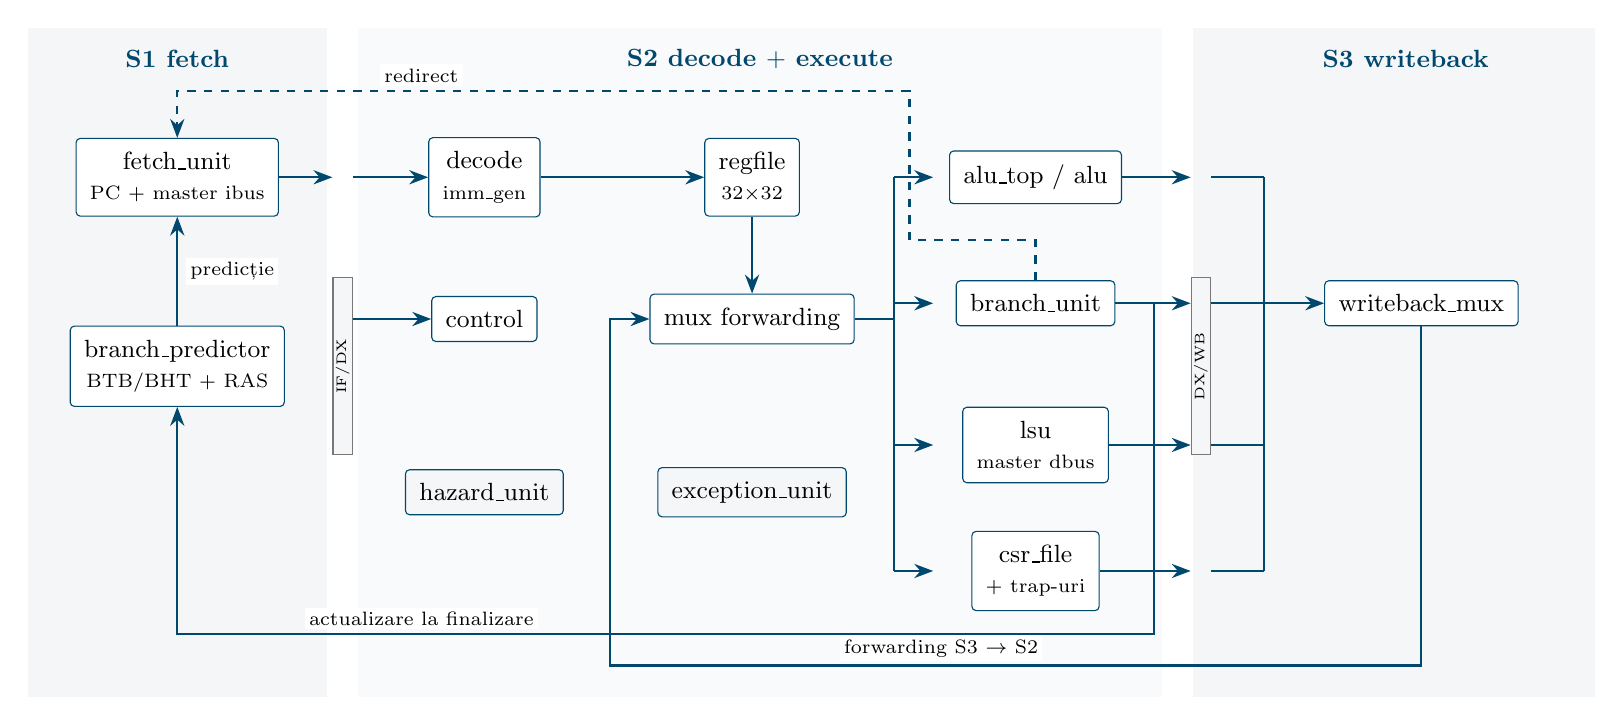
\begin{tikzpicture}[x=1mm,y=1mm,font=\small]

  % --- benzile stagiilor --------------------------------------------------
  \begin{scope}[on background layer]
    \fill[boxbg]     (-16,-72) rectangle (22,13);
    \fill[boxbg!55]  (26,-72)  rectangle (128,13);
    \fill[boxbg]     (132,-72) rectangle (183,13);
  \end{scope}
  \node[font=\small\bfseries,color=accent] at (3,9)   {S1 fetch};
  \node[font=\small\bfseries,color=accent] at (77,9)  {S2 decode $+$ execute};
  \node[font=\small\bfseries,color=accent] at (159,9) {S3 writeback};

  % --- S1 -----------------------------------------------------------------
  \node[blk,minimum width=32,minimum height=12] (fu) at (3,-6)
        {fetch\_unit\\\scriptsize PC $+$ master ibus};
  \node[blk,minimum width=32,minimum height=12] (bp) at (3,-30)
        {branch\_predictor\\\scriptsize BTB/BHT $+$ RAS};

  % --- registrele dintre stagii -------------------------------------------
  \node[draw=rulegrey,fill=boxbg,minimum width=7,minimum height=64,inner sep=0] (ifdx) at (24,-30) {};
  \node[rotate=90,font=\tiny] at (24,-30) {IF/DX};
  \node[draw=rulegrey,fill=boxbg,minimum width=7,minimum height=64,inner sep=0] (dxwb) at (133,-30) {};
  \node[rotate=90,font=\tiny] at (133,-30) {DX/WB};

  % --- calea de date din S2 -----------------------------------------------
  \node[blk,minimum width=24,minimum height=12] (dec) at (42,-6)
        {decode\\\scriptsize imm\_gen};
  \node[blk,minimum width=24,minimum height=9]  (ctl) at (42,-24) {control};
  \node[blk,minimum width=24,minimum height=12] (rf)  at (76,-6)
        {regfile\\\scriptsize 32$\times$32};
  \node[blk,minimum width=24,minimum height=9]  (fwd) at (76,-24) {mux forwarding};

  \node[blk,minimum width=26,minimum height=10] (alu) at (112,-6)  {alu\_top / alu};
  \node[blk,minimum width=26,minimum height=10] (bu)  at (112,-22) {branch\_unit};
  \node[blk,minimum width=26,minimum height=11] (lsu) at (112,-40)
        {lsu\\\scriptsize master dbus};
  \node[blk,minimum width=26,minimum height=11] (csr) at (112,-56)
        {csr\_file\\\scriptsize $+$ trap-uri};

  \node[blkf,minimum width=28,minimum height=9] (hz)  at (42,-46) {hazard\_unit};
  \node[blkf,minimum width=30,minimum height=9] (exc) at (76,-46) {exception\_unit};

  % --- S3 -----------------------------------------------------------------
  \node[blk,minimum width=30,minimum height=10] (wb) at (161,-22) {writeback\_mux};

  % --- legături -----------------------------------------------------------
  \draw[flow] (fu.east) -- (ifdx.west|-fu);
  \draw[flow] (ifdx.east|-dec) -- (dec.west);
  \draw[flow] (ifdx.east|-ctl) -- (ctl.west);
  \draw[flow] (dec.east) -- (rf.west);
  \draw[flow] (rf.south) -- (fwd.north);

  % magistrala de operanzi
  \draw[flow,-] (fwd.east) -- (94,-24);
  \draw[thick,draw=accent] (94,-6) -- (94,-56);
  \foreach \y in {-6,-22,-40,-56} \draw[flow] (94,\y) -- (99,\y);

  \draw[flow] (alu.east) -- (dxwb.west|-alu);
  \draw[flow] (bu.east)  -- (dxwb.west|-bu);
  \draw[flow] (lsu.east) -- (dxwb.west|-lsu);
  \draw[flow] (csr.east) -- (dxwb.west|-csr);

  % magistrala de rezultate
  \draw[flow,-] (dxwb.east|-alu) -- (141,-6);
  \draw[flow,-] (dxwb.east|-bu)  -- (141,-22);
  \draw[flow,-] (dxwb.east|-lsu) -- (141,-40);
  \draw[flow,-] (dxwb.east|-csr) -- (141,-56);
  \draw[thick,draw=accent] (141,-6) -- (141,-56);
  \draw[flow] (141,-22) -- (wb.west);

  % predictorul: consultare în sus, actualizare pe la bază
  \draw[flow] (bp.north) -- (fu.south) node[lbl,midway,right=1mm]{predicție};
  \draw[flow] (127,-22) -- (127,-64) -- (3,-64) -- (bp.south);
  \node[lbl,above=0.5mm] at (34,-64) {actualizare la finalizare};

  % redirectarea fluxului la branch prezis greșit
  \draw[flowd] (bu.north) -- (112,-14) -- (96,-14) -- (96,5) -- (3,5) -- (fu.north);
  \node[lbl,above=0.5mm] at (34,5) {redirect};

  % valoarea scrisă înapoi în muxul de forwarding
  \draw[flow] (wb.south) -- (161,-68) -- (58,-68) -- (58,-24) -- (fwd.west);
  \node[lbl,above=0.5mm] at (100,-68) {forwarding S3 $\to$ S2};
\end{tikzpicture}}
\caption{Structura procesorului. Fiecare cutie este un modul separat, cu
excepția muxului de forwarding, care este logică inline la nivelul de vârf.
Am ținut modulele mici și cu o singură responsabilitate, tocmai ca fiecare să
poată fi verificat separat --- ALU-ul și predictorul au testbench-uri proprii.}
\label{fig:cpu}
\end{figure}

Portul extern este o intrare de ceas, un reset, cele două porturi master
AXI4-Lite și cele șase semnale ale interfeței cu controlerul de întreruperi ---
cererea, numărul sursei oferite, setul de surse în așteptare, masca procesorului,
confirmarea și terminarea --- plus un semnal de observabilitate care spune dacă
un trap este deschis. Instrucțiunea de așteptare, stiva adreselor de retur și
contoarele de performanță se văd toate prin această listă, fără niciun semnal
propriu. Este o constrângere pe care mi-am
impus-o deliberat: procesorul este un bloc între altele, într-un sistem construit
în paralel de alți doi oameni, iar orice semnal adăugat la interfață ar fi cerut
o modificare la ei.

\section{Fetch-ul instrucțiunilor și predicția branch-urilor}

Unitatea de fetch este master pe magistrala de instrucțiuni și menține o
singură tranzacție în curs. Am reprezentat-o prin trei semnale de stare, nu
printr-un registru de stare: „cererea de adresă este emisă și neacceptată”,
„citirea este în curs” și „instrucțiunea care vine trebuie aruncată”.

Al treilea vine dintr-o restricție a protocolului. O citire AXI
\textbf{nu poate fi anulată} după ce semnalul de validare al adresei a fost
ridicat. Când predictorul greșește și pipeline-ul trebuie redirecționat, cererea
deja emisă nu poate fi retrasă --- singura soluție corectă este să lași
răspunsul să vină și să-l ignori. De aceea semnalul de aruncare este un indicator
ortogonal, nu o a patra stare: poate fi armat din oricare dintre cele două stări
ocupate.

\begin{figure}[H]
\centering
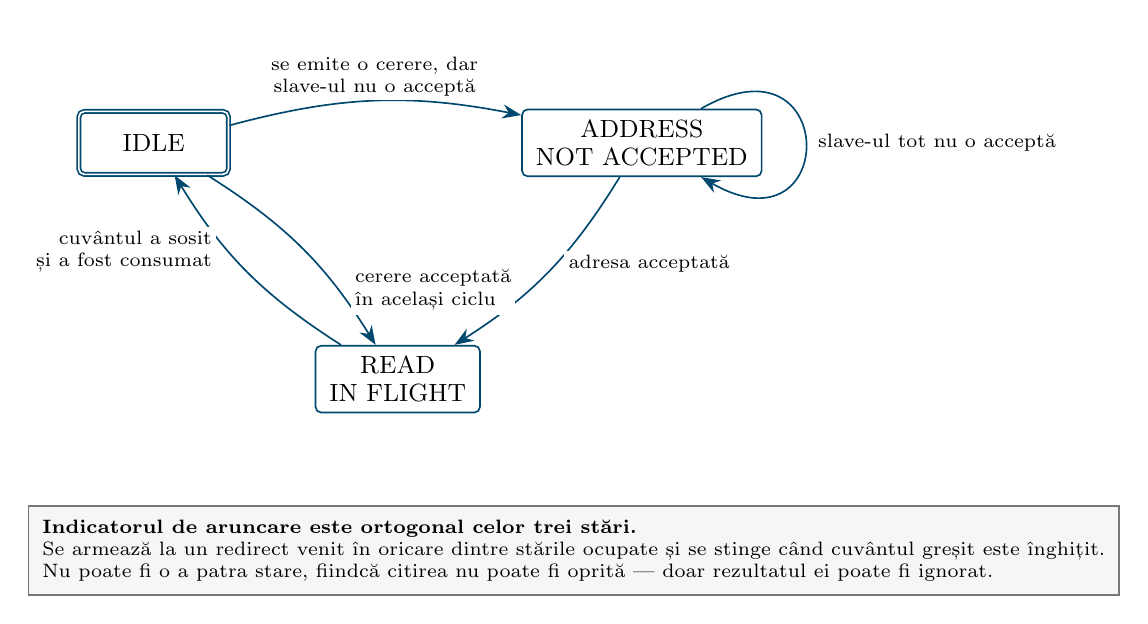
\begin{tikzpicture}[x=1mm,y=1mm,>={Stealth[length=2.4mm]},semithick]
  \node[stbi] (idle) at (0,0)    {IDLE};
  \node[stb]  (arp)  at (62,0)   {ADDRESS\\[-1pt]NOT ACCEPTED};
  \node[stb]  (infl) at (31,-30) {READ\\[-1pt]IN FLIGHT};

  \draw[->,draw=accent] (idle) to[bend left=13]
      node[lbl,above,align=center,pos=0.5]
      {se emite o cerere, dar\\\scriptsize slave-ul nu o acceptă} (arp);
  \draw[->,draw=accent,looseness=6,out=30,in=-30] (arp) to
      node[lbl,right=1mm]{\scriptsize slave-ul tot nu o acceptă} (arp);
  \draw[->,draw=accent] (arp) to[bend left=13]
      node[lbl,right=1mm,align=left,pos=0.45]{adresa acceptată} (infl);
  \draw[->,draw=accent] (infl) to[bend left=13]
      node[lbl,left=1.5mm,align=right,pos=0.62]
      {cuvântul a sosit\\\scriptsize și a fost consumat} (idle);
  \draw[->,draw=accent] (idle) to[bend left=13]
      node[lbl,right=1.5mm,align=left,pos=0.74]
      {cerere acceptată\\\scriptsize în același ciclu} (infl);

  \node[align=left,font=\scriptsize,anchor=north west,
        draw=rulegrey,fill=boxbg,inner sep=5pt] at (-16,-46)
    {\textbf{Indicatorul de aruncare este ortogonal celor trei stări.}\\
     Se armează la un redirect venit în oricare dintre stările ocupate și
     se stinge când cuvântul greșit este înghițit.\\
     Nu poate fi o a patra stare, fiindcă citirea nu poate fi oprită ---
     doar rezultatul ei poate fi ignorat.};
\end{tikzpicture}
\caption{Comportamentul slotului de citire. Niciunul dintre cele trei nume nu
există ca registru de stare în circuit: ele sunt produse de trei indicatoare
independente. Contururile duble marchează starea de după reset.}
\label{fig:fetchfsm}
\end{figure}

Predictorul folosește un tabel de 128 de intrări care combină ținta branch-ului cu
un contor de direcție, plus o stivă separată de 8 adrese pentru revenirile din
funcții. Stiva există pentru că un return are aproape întotdeauna o altă
țintă decât data trecută, deci tabelul obișnuit nu îl poate prezice; adresa de
retur, în schimb, este cunoscută exact în momentul apelului.

\section{Controlul pipeline-ului}
\label{sec:pipectl}

\subsection{Registrele dintre stagii și bubble-urile}

Ambele registre dintre stagii --- IF/DX și DX/WB --- sunt construite la fel: un
bit de validitate plus sarcina utilă. Bitul de validitate este ceea ce face o
bubble sigur: nimic în aval nu se uită la sarcina utilă dacă bitul este zero,
deci un bubble înseamnă pur și simplu \emph{valid}~=~0, iar un flush produce o
instrucțiune nulă garantată, indiferent ce conțin biții de date.

Alternativa ar fi fost injectarea codului unei instrucțiuni care nu face nimic.
Aceea ar fi cerut ca traseul de flush să producă 32 de biți corecți și ca
fiecare decodor din aval să îi interpreteze --- mai mult hardware și mai multe
feluri de a greși. Sarcina utilă se încarcă doar când o instrucțiune reală
avansează, deci bubble-urile și stall-urile lasă bistabilele liniștite.

\subsection{Unitatea de hazarduri}

Toate deciziile de stall, de flush și de forwarding al operanzilor se iau
într-un singur modul. Niciun stagiu nu își gestionează singur avansul, iar
controlul întreg încape în câteva ecuații combinaționale. Consecința practică
este că nu există nicio mașină de stări care să conducă pipeline-ul --- ceea ce
înseamnă și că nu există stări nevalide în care el să ajungă.

\begin{table}[H]
\centering
\caption{Sursele de stall și de flush}
\label{tab:hazsurse}
\small
\begin{tabular}{@{}L{0.20\linewidth}L{0.70\linewidth}@{}}
\toprule
\textbf{Categorie} & \textbf{Surse} \\
\midrule
Stall (două) &
  O tranzacție de date în curs pe magistrală, și o instrucțiune de așteptare
  adormită. Atât. Un fetch de instrucțiune care nu este gata \emph{nu}
  creează un stall în stagiul doi: produce un bubble, adică stagiul avansează, doar că fără
  instrucțiune. \\
\addlinespace
Flush (trei) &
  Predicție greșită rezolvată în S2, intrare în trap, și revenire din trap.
  Toate trei fac același lucru --- ridică semnalul de redirect și încarcă
  un bubble în registrul dintre stagii --- deci există un singur mecanism, nu
  trei. \\
\bottomrule
\end{tabular}
\end{table}

Hazardul clasic ,,încărcare urmată de folosire'' nu există aici. Într-un
pipeline cu trei stagii, datele unei încărcări sunt deja în S3 în momentul în
care instrucțiunea care le consumă intră în S2, deci o singură cale de
forwarding S3~$\rightarrow$~S2 le acoperă, fără niciun ciclu pierdut.

\paragraph{Când stall-ul și flush-ul cer lucruri diferite, flush-ul câștigă}, fiindcă
tocmai invalidează instrucțiunea pe care stall-ul o aștepta. Regula are însă o a
doua jumătate, care vine din același semnal: fiecare condiție de flush este
condiționată de avansul stagiului doi, deci un trap \emph{nu poate} părăsi S2
cât timp o tranzacție de date este încă în curs. Magistrala nu rămâne niciodată
cu o tranzacție orfană, al cărei răspuns nu îl mai așteaptă nimeni.

\subsection{Ordinea deciziilor în stagiul doi}

Toate deciziile arhitecturale se iau în S2, într-o ordine fixă:

\begin{center}
întrerupere \; $>$ \; excepție sincronă \; $>$ \; revenire din trap \; $>$ \;
predicție greșită
\end{center}

Întreruperea este testată prima, și anume \emph{înainte} ca instrucțiunea să
emită vreo tranzacție de date, ca instrucțiunea întreruptă să poată fi reluată
identic după ce rutina de tratare se întoarce. O excepție trece înaintea unei
predicții greșite pentru că o instrucțiune care a dat fault nu mai are niciun
drum corect de urmat.

\subsection{Ce costă fiecare caz}

\begin{figure}[H]
\centering
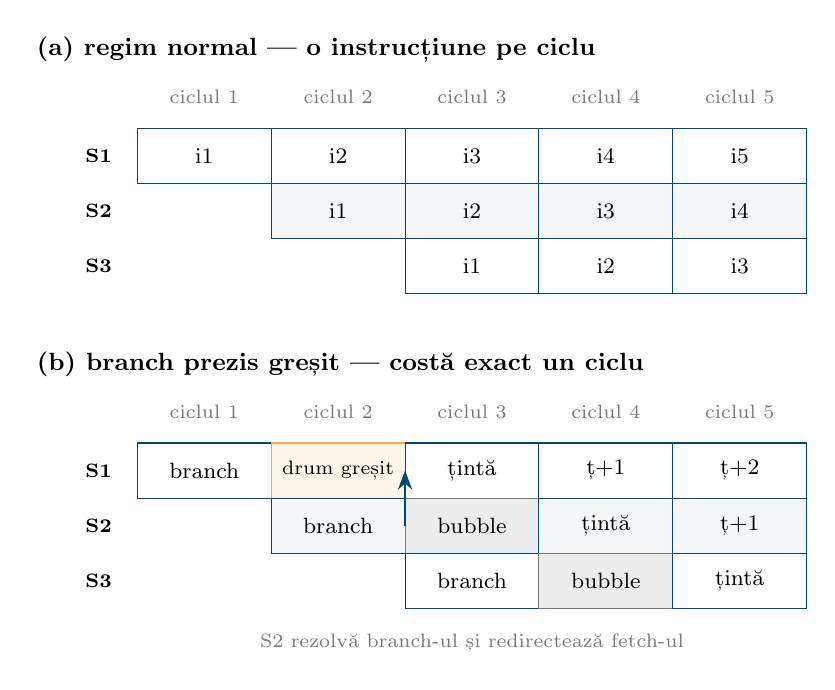
\begin{tikzpicture}[x=1mm,y=1mm,font=\footnotesize]
  \def\cw{17}\def\rh{7}

  % ---------------- panoul A: regim normal ----------------
  \node[font=\small\bfseries,anchor=west] at (-14,10) {(a) regim normal --- o instrucțiune pe ciclu};
  \foreach \c/\lbl in {0/1,1/2,2/3,3/4,4/5}
    \node[font=\scriptsize,color=rulegrey] at (\c*\cw+\cw/2,4) {ciclul \lbl};
  \foreach \r/\st in {0/S1,1/S2,2/S3}
    \node[font=\scriptsize\bfseries,anchor=east] at (-2,-\r*\rh-\rh/2) {\st};

  \foreach \c/\t in {0/i1,1/i2,2/i3,3/i4,4/i5}
    \node[draw=accent,fill=white,minimum width=\cw mm,minimum height=\rh mm,inner sep=0]
      at (\c*\cw+\cw/2,-\rh/2) {\t};
  \foreach \c/\t in {1/i1,2/i2,3/i3,4/i4}
    \node[draw=accent,fill=boxbg,minimum width=\cw mm,minimum height=\rh mm,inner sep=0]
      at (\c*\cw+\cw/2,-\rh-\rh/2) {\t};
  \foreach \c/\t in {2/i1,3/i2,4/i3}
    \node[draw=accent,fill=white,minimum width=\cw mm,minimum height=\rh mm,inner sep=0]
      at (\c*\cw+\cw/2,-2*\rh-\rh/2) {\t};

  % ---------------- panoul B: predicție greșită ----------------
  \begin{scope}[yshift=-40mm]
  \node[font=\small\bfseries,anchor=west] at (-14,10)
    {(b) branch prezis greșit --- costă exact un ciclu};
  \foreach \c/\lbl in {0/1,1/2,2/3,3/4,4/5}
    \node[font=\scriptsize,color=rulegrey] at (\c*\cw+\cw/2,4) {ciclul \lbl};
  \foreach \r/\st in {0/S1,1/S2,2/S3}
    \node[font=\scriptsize\bfseries,anchor=east] at (-2,-\r*\rh-\rh/2) {\st};

  \node[draw=accent,fill=white,minimum width=\cw mm,minimum height=\rh mm,inner sep=0]
    at (0*\cw+\cw/2,-\rh/2) {branch};
  \node[draw=orange!70,fill=warnbg,minimum width=\cw mm,minimum height=\rh mm,inner sep=0]
    at (1*\cw+\cw/2,-\rh/2) {\scriptsize drum greșit};
  \foreach \c/\t in {2/țintă,3/ț+1,4/ț+2}
    \node[draw=accent,fill=white,minimum width=\cw mm,minimum height=\rh mm,inner sep=0]
      at (\c*\cw+\cw/2,-\rh/2) {\t};

  \node[draw=accent,fill=boxbg,minimum width=\cw mm,minimum height=\rh mm,inner sep=0]
    at (1*\cw+\cw/2,-\rh-\rh/2) {branch};
  \node[draw=rulegrey,fill=black!7,minimum width=\cw mm,minimum height=\rh mm,inner sep=0]
    at (2*\cw+\cw/2,-\rh-\rh/2) {bubble};
  \foreach \c/\t in {3/țintă,4/ț+1}
    \node[draw=accent,fill=boxbg,minimum width=\cw mm,minimum height=\rh mm,inner sep=0]
      at (\c*\cw+\cw/2,-\rh-\rh/2) {\t};

  \node[draw=accent,fill=white,minimum width=\cw mm,minimum height=\rh mm,inner sep=0]
    at (2*\cw+\cw/2,-2*\rh-\rh/2) {branch};
  \node[draw=rulegrey,fill=black!7,minimum width=\cw mm,minimum height=\rh mm,inner sep=0]
    at (3*\cw+\cw/2,-2*\rh-\rh/2) {bubble};
  \node[draw=accent,fill=white,minimum width=\cw mm,minimum height=\rh mm,inner sep=0]
    at (4*\cw+\cw/2,-2*\rh-\rh/2) {țintă};

  % redirectarea: din celula care rezolvă branch-ul, în sus, la fetch-ul corect
  \draw[flow] (2*\cw,-\rh-\rh/2) -- (2*\cw,-\rh/2);
  \node[font=\scriptsize,anchor=north,color=rulegrey] at (2.5*\cw,-3*\rh-2)
    {S2 rezolvă branch-ul și redirectează fetch-ul};
  \end{scope}
\end{tikzpicture}
\caption{Ocuparea stagiilor, ciclu cu ciclu. În regim normal o instrucțiune
intră în S2 în fiecare ciclu. La o predicție greșită, instrucțiunea de pe drumul
greșit este aruncată, S2 execută un bubble, iar instrucțiunea corectă ajunge în S2
la două cicluri după branch --- un singur ciclu pierdut.}
\label{fig:pipeocc}
\end{figure}

\begin{table}[H]
\centering
\caption{Cele patru cazuri care determină debitul}
\label{tab:cputiming}
\small
\begin{tabular}{@{}L{0.22\linewidth}L{0.68\linewidth}@{}}
\toprule
\textbf{Caz} & \textbf{Comportament} \\
\midrule
Operație ALU & O instrucțiune intră în S2 în fiecare ciclu; un ciclu per
  instrucțiune, măsurat pe cod liniar cu memorie de instrucțiuni cu latență de
  un ciclu. \\
Încărcare / stocare & S2 se blochează pe toată durata tranzacției pe magistrală.
  S1 poate termina un fetch deja pornit și îl parchează; nimic nu intră și
  nimic nu iese din S2. \\
Predicție greșită & Costă exact un ciclu, ca în Figura~\ref{fig:pipeocc}. \\
Intrare în trap & Niciun ciclu peste redirect. Instrucțiunea care a dat
  fault este anulată pe drumul ei către registrul următor, în același ciclu în
  care starea de trap este scrisă. \\
\bottomrule
\end{tabular}
\end{table}

\subsection{Forwarding-ul operanzilor}

Unitatea de hazarduri calculează și potrivirile de forwarding: registrul
destinație din S3 comparat cu fiecare registru sursă din S2, cu registrul zero
exclus. O potrivire înlocuiește valoarea citită din fișierul de registre cu
valoarea care se scrie.

\section{Unitatea load/store și porturile AXI4-Lite}
\label{sec:lsu}

Unitatea load/store conține singura mașină de stări codificată explicit în
procesor. Am ținut-o deliberat minimală --- trei stări --- pentru că restul
complexității stă în urmărirea handshake-urilor, nu în stare.

\begin{figure}[H]
\centering
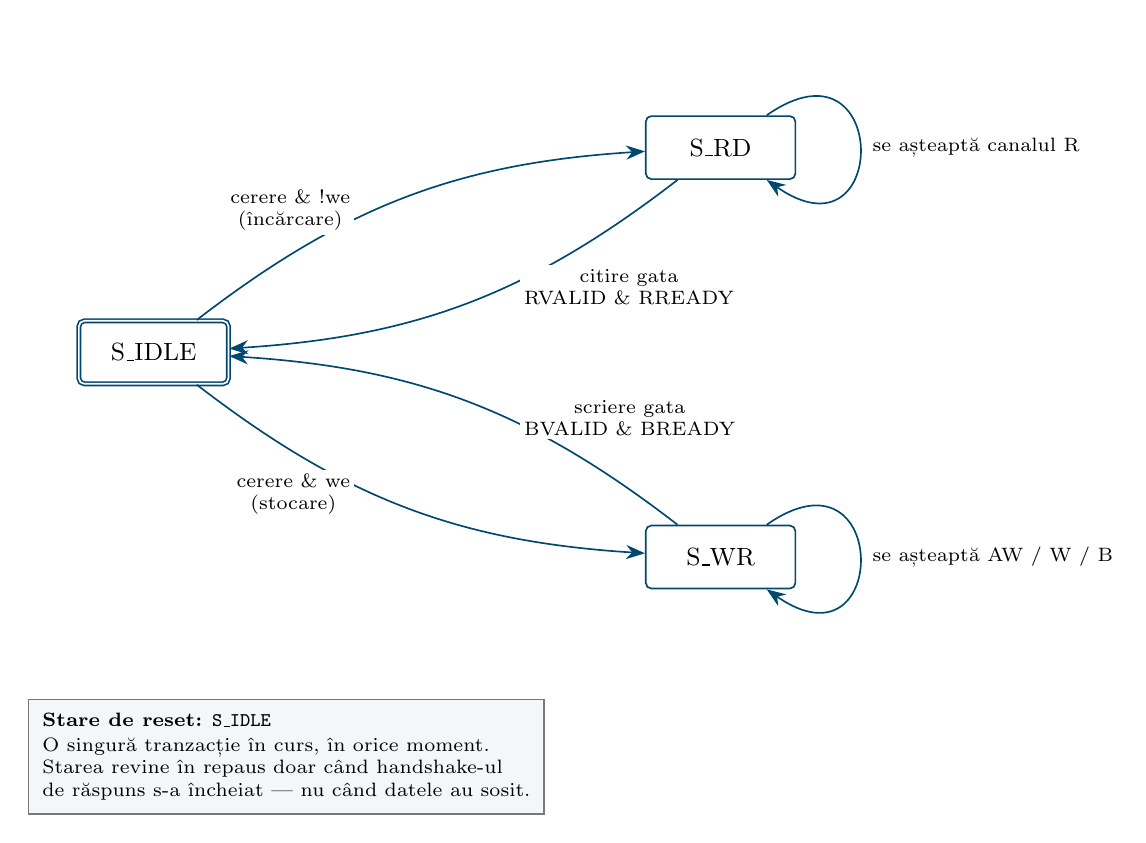
\begin{tikzpicture}[x=1mm,y=1mm,>={Stealth[length=2.4mm]},semithick]
  \node[stbi] (idle) at (0,0)    {S\_IDLE};
  \node[stb]  (rd)   at (72,26)  {S\_RD};
  \node[stb]  (wr)   at (72,-26) {S\_WR};

  \draw[->,draw=accent] (idle) to[bend left=17]
      node[lbl,pos=0.30,above left=0mm and -4mm,align=center]
      {cerere \&\ !we\\\scriptsize (încărcare)} (rd);
  \draw[->,draw=accent] (rd) to[bend left=17]
      node[lbl,pos=0.30,below right=0mm and -4mm,align=center]
      {citire gata\\\scriptsize RVALID \&\ RREADY} (idle);

  \draw[->,draw=accent] (idle) to[bend right=17]
      node[lbl,pos=0.30,below left=0mm and -4mm,align=center]
      {cerere \&\ we\\\scriptsize (stocare)} (wr);
  \draw[->,draw=accent] (wr) to[bend right=17]
      node[lbl,pos=0.30,above right=0mm and -4mm,align=center]
      {scriere gata\\\scriptsize BVALID \&\ BREADY} (idle);

  \draw[->,draw=accent] (rd) to[out=35,in=-35,looseness=6]
      node[lbl,right=1mm]{\scriptsize se așteaptă canalul R} (rd);
  \draw[->,draw=accent] (wr) to[out=35,in=-35,looseness=6]
      node[lbl,right=1mm]{\scriptsize se așteaptă AW / W / B} (wr);

  \node[align=left,font=\scriptsize,anchor=north west,
        draw=rulegrey,fill=boxbg,inner sep=5pt] at (-16,-44)
    {\textbf{Stare de reset:} \texttt{S\_IDLE}\\[1pt]
     O singură tranzacție în curs, în orice moment.\\
     Starea revine în repaus doar când handshake-ul\\
     de răspuns s-a încheiat --- nu când datele au sosit.};
\end{tikzpicture}
\caption{Mașina de stări a unității load/store. Cele două bucle pe loc nu sunt
decorative: ele sunt cazul obișnuit, pentru că un slave poate întârzia oricât.}
\label{fig:lsufsm}
\end{figure}

Starea singură nu spune cât de departe a ajuns o tranzacție, pentru că o scriere
are \textbf{trei canale independente}: adresa, datele și răspunsul. Adresa poate
fi acceptată înaintea datelor sau invers. De aceea am adăugat trei indicatoare
separate, câte unul per canal, iar starea revine în repaus doar când toate trei
s-au închis. Aceasta a fost lecția practică cea mai directă despre AXI: nu
există un singur semnal „gata”, iar a presupune o ordine între canale este
exact felul în care un master pare corect până când întâlnește un slave mai
lent.

\begin{figure}[H]
\centering
\begin{tikztimingtable}[timing/slope=0,timing/coldist=2pt,xscale=1.05]
  clk        & 12{C} \\
  ARVALID    & 2L 2H 8L \\
  ARREADY    & 2L 2H 8L \\
  ARADDR     & 2U 2D{adresa} 8U \\
  RVALID     & 6L 2H 4L \\
  RREADY     & 4L 4H 4L \\
  RDATA      & 6U 2D{date} 4U \\
  S2 blocat  & 2L 6H 4L \\
  \extracode
  \begin{pgfonlayer}{background}
    \vertlines[help lines]{2,4,6,8}
  \end{pgfonlayer}
\end{tikztimingtable}
\caption{O încărcare pe magistrala de date, cu un slave care răspunde în două
cicluri. Disponibilitatea pe canalul de date se ridică abia după ce adresa a
fost acceptată, iar stagiul doi rămâne blocat până când cuvântul este preluat
--- nu până când sosește.}
\label{fig:lsuread}
\end{figure}

\begin{figure}[H]
\centering
\begin{tikztimingtable}[timing/slope=0,timing/coldist=2pt,xscale=1.05]
  clk        & 12{C} \\
  AWVALID    & 2L 2H 8L \\
  AWREADY    & 2L 2H 8L \\
  WVALID     & 2L 4H 6L \\
  WREADY     & 4L 2H 6L \\
  WSTRB      & 2U 4D{mască} 6U \\
  BVALID     & 8L 2H 2L \\
  BREADY     & 6L 4H 2L \\
  \extracode
  \begin{pgfonlayer}{background}
    \vertlines[help lines]{2,4,6,8,10}
  \end{pgfonlayer}
\end{tikztimingtable}
\caption{O stocare unde slave-ul acceptă adresa înaintea datelor. Acesta este
cazul pentru care există cele trei indicatoare: disponibilitatea pe canalul de
răspuns se ridică abia după ce \emph{amândouă} handshake-urile, de adresă și de
date, s-au încheiat.}
\label{fig:lsuwrite}
\end{figure}

\paragraph{Măștile pe octet.} O stocare de octet sau de jumătate de cuvânt se
face prin măștile \sig{WSTRB}, nu prin citire-modificare-scriere. Unitatea
calculează masca din dimensiunea accesului și din cei doi biți de jos ai
adresei. Un acces nealiniat nu este emis deloc pe magistrală: este oprit în
procesor și produce o excepție precisă, cu adresa care a greșit salvată în
registrul dedicat.

\section{Registrele de control, trap-urile și întreruperile}

Am implementat registrele de control și stare în măsura cerută de un sistem cu
întreruperi: starea globală de trap, activarea per sursă, vectorul de trap,
adresa de retur, cauza, valoarea asociată, identificarea implementării și
contoarele de performanță.

\subsection{Urmărirea nivelurilor de trap}

Nucleul ține \textbf{câte un bit pentru fiecare nivel de trap deschis}, pe o
stivă adâncă de 16 --- exact numărul maxim de niveluri pe care controlerul de
întreruperi le acceptă. Bitul spune ce fel de trap a deschis nivelul:
\texttt{1} pentru o întrerupere, \texttt{0} pentru o excepție sincronă. Fiecare
trap acceptat pune un bit, fiecare revenire scoate unul, iar semnalul de
terminare pleacă spre controlerul de întreruperi numai dacă bitul scos este
\texttt{1}.

Un singur indicator „suntem într-o întrerupere”, ridicat la orice întrerupere și
coborât la orice revenire, ar părea suficient, dar nu ar putea deosebi două
situații:

\begin{itemize}[itemsep=3pt,topsep=3pt]
\item \textbf{Două rutine imbricate.} Amândouă revin, dar un indicator unic ar
      produce un singur semnal de terminare în loc de două, iar nivelul exterior
      ar rămâne deschis pentru totdeauna în stiva controlerului, cu sursa lui
      blocată.
\item \textbf{O excepție sincronă în interiorul unei rutine de tratare.}
      Revenirea din excepție ar trimite semnalul de terminare al întreruperii,
      închizând-o în timp ce rutina ei încă rulează.
\end{itemize}

Stiva de biți de fel deosebește ambele cazuri fără logică suplimentară: felul
trap-ului care se închide este chiar bitul scos de pe stivă.

\begin{figure}[H]
\centering
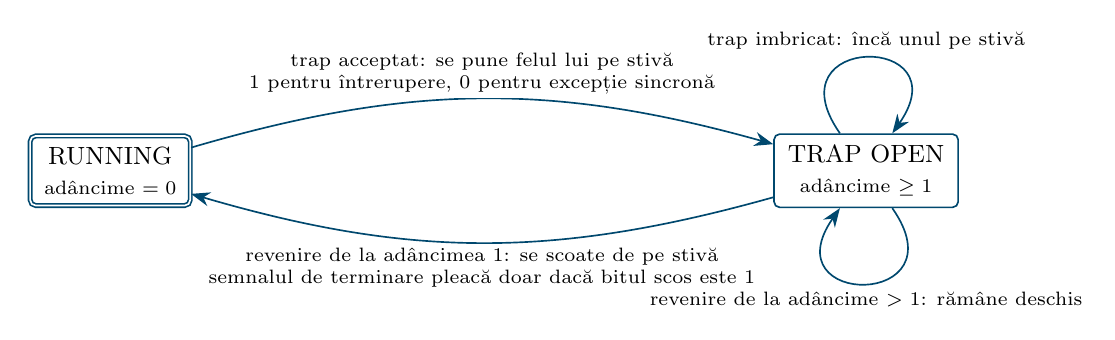
\begin{tikzpicture}[x=1mm,y=1mm,>={Stealth[length=2.4mm]},semithick]
  \node[stbi] (run)  at (0,0)   {RUNNING\\\scriptsize adâncime $=0$};
  \node[stb]  (open) at (96,0)  {TRAP OPEN\\\scriptsize adâncime $\ge 1$};

  \draw[->,draw=accent] (run) to[bend left=16]
    node[lbl,pos=0.5,above,align=center]
    {trap acceptat: se pune felul lui pe stivă\\
     \scriptsize 1 pentru întrerupere, 0 pentru excepție sincronă} (open);

  \draw[->,draw=accent] (open) to[bend left=16]
    node[lbl,pos=0.5,below,align=center]
    {revenire de la adâncimea 1: se scoate de pe stivă\\
     \scriptsize semnalul de terminare pleacă doar dacă bitul scos este 1} (run);

  \draw[->,draw=accent,looseness=6,out=125,in=55] (open) to
    node[lbl,above=0.5mm,align=center]{trap imbricat: încă unul pe stivă} (open);

  \draw[->,draw=accent,looseness=6,out=-55,in=-125] (open) to
    node[lbl,below=0.5mm,align=center]{revenire de la adâncime $>1$: rămâne deschis} (open);
\end{tikzpicture}
\caption{Urmărirea trap-urilor în procesor. Nivelurile deschise formează o stivă
de biți de fel, nu o pereche de indicatoare: fiecare trap pune un bit, fiecare
revenire scoate unul. Astfel, o excepție apărută într-o rutină de întrerupere se
întoarce fără să anunțe terminarea întreruperii, iar fiecare nivel imbricat își
trimite propriul semnal de terminare.}
\label{fig:trapfsm}
\end{figure}

\subsection{Cauzele de trap}

Cauzele sunt evaluate într-un lanț de prioritate fix, nu în ordinea numerică a
codurilor lor. Ordinea contează atunci când două condiții sunt adevărate în
același ciclu --- de exemplu o instrucțiune ilegală la o adresă nealiniată --- și
am ales-o astfel încât cauza raportată să fie cea care a apărut prima în
execuția instrucțiunii.

\begin{table}[H]
\centering
\caption{Cauzele de trap implementate și valoarea salvată pentru fiecare}
\label{tab:trapcauses}
\small
\begin{tabular}{@{}L{0.34\linewidth}L{0.52\linewidth}@{}}
\toprule
\textbf{Cauză} & \textbf{Valoarea asociată salvată} \\
\midrule
Întrerupere externă & --- (numărul sursei intră în codul cauzei) \\
Adresă de instrucțiune nealiniată & adresa țintă calculată \\
Eroare de acces la instrucțiune & adresa care a produs eroarea pe magistrală \\
Instrucțiune ilegală & cuvântul de instrucțiune în sine \\
Punct de întrerupere software & adresa instrucțiunii \\
Adresă de încărcare / stocare nealiniată & adresa efectivă calculată \\
Eroare de acces la încărcare / stocare & adresa care a primit eroare \\
Apel de mediu din modul mașină & --- \\
\bottomrule
\end{tabular}
\end{table}

\paragraph{Instrucțiunea de așteptare.} Instrucțiunea \sig{WFI} oprește
fetch-ul de instrucțiuni până la sosirea unei întreruperi. Am implementat-o
astfel încât magistrala de instrucțiuni să tacă efectiv pe durata așteptării ---
nu doar să ignore rezultatele --- pentru că într-un sistem real acesta este
singurul mod în care oprirea are vreun sens. Este și mecanismul pe care se
sprijină testul de sistem: procesorul programează DMA-ul, execută \sig{WFI}, și
este trezit de întreruperea de terminare a transferului.

% ===========================================================================
\chapter{Temporizatorul de sistem}
\label{ch:mtimer}

Temporizatorul este cel mai mic dintre blocurile pe care le-am proiectat și,
din punctul de vedere al sistemului, este doar încă o sursă de întrerupere ---
dar este sursa care face posibilă orice formă de programare în timp.

\section{Contorul și comparația}

Implementează perechea clasică din specificația RISC-V: un contor
liber de 64 de biți care numără cicluri, și un registru de comparație de 64 de
biți. Când contorul atinge sau depășește comparația, linia de întrerupere se
ridică și rămâne sus până când software-ul mută comparația mai departe.

Linia de întrerupere intră în controlerul de întreruperi pe sursa 7.

Ambele registre sunt de 64 de biți, dar magistrala este de 32, deci fiecare se
accesează în două jumătăți. De aici vin cele două subtilități ale blocului, una
la scriere și una la citire.

\section{Armarea fără declanșare falsă}

\begin{figure}[H]
\centering
\begin{tikztimingtable}[timing/slope=0,timing/coldist=2pt,xscale=1.0]
  clk                    & 14{C} \\
  comparație, jumăt. jos & 4D{FFFFFFFF} 10D{țintă\_jos} \\
  comparație, jumăt. sus & 8D{FFFFFFFF} 6D{țintă\_sus} \\
  contor $\ge$ comparație & 12L 2H \\
  întrerupere            & 14{L} \\
  \extracode
  \begin{pgfonlayer}{background}
    \vertlines[help lines]{4,8,12}
  \end{pgfonlayer}
\end{tikztimingtable}
\caption{Secvența corectă de armare. Cât timp jumătatea superioară este încă
numai de unu, comparația nu poate trece, deci scrierea jumătății inferioare mai
întâi este sigură. În ordinea inversă există o fereastră între cele două scrieri
în care o jumătate veche poate declanșa o întrerupere falsă.}
\label{fig:tmrarm}
\end{figure}

Ordinea sigură este deci: jumătatea inferioară, apoi cea superioară. Am
documentat-o ca parte a contractului blocului, nu ca recomandare --- este genul
de detaliu care, nescris, produce un defect care apare o dată la câteva mii de
armări și nu se reproduce niciodată la cerere.

\section{Citirea contorului din software pe 32 de biți}

Aceeași problemă apare simetric la \emph{citirea} contorului: jumătatea
inferioară se poate rostogoli între cele două tranzacții de magistrală. Soluția
uzuală, pe care software-ul de test o folosește, este să citească jumătatea
superioară, apoi cea inferioară, apoi din nou cea superioară, și să reia dacă
prima și ultima diferă.

% ===========================================================================
\chapter{Controlerul de întreruperi}
\label{ch:pic}

\section{De ce are nevoie sistemul de un asemenea bloc}

Procesorul primește, la un moment dat, o singură cerere de întrerupere, însoțită de numărul
sursei care a produs-o. Sistemul are însă șase surse hardware conectate --- patru
canale DMA, memoria duală și temporizatorul --- plus canalele software. Ceva
trebuie să decidă care dintre ele ajunge la nucleu, în ce ordine, și ce se
întâmplă când una mai urgentă apare în timp ce alta este deja tratată.

Am proiectat controlerul pentru \textbf{16 surse hardware și 16 canale
software}, adică 32 de surse logice care intră în același lanț de rezoluție. O
cerere software se contopește cu slotul hardware corespunzător, deci odată
intrată în lanț este indistinguibilă de una hardware: aceeași prioritate, același
termen limită, același comportament la imbricare. Aceasta a fost o decizie
conștientă --- alternativa, un lanț separat pentru software, ar fi dublat logica
de rezoluție fără niciun câștig.

\section{Structura internă}

\begin{figure}[H]
\centering
\resizebox{\linewidth}{!}{%
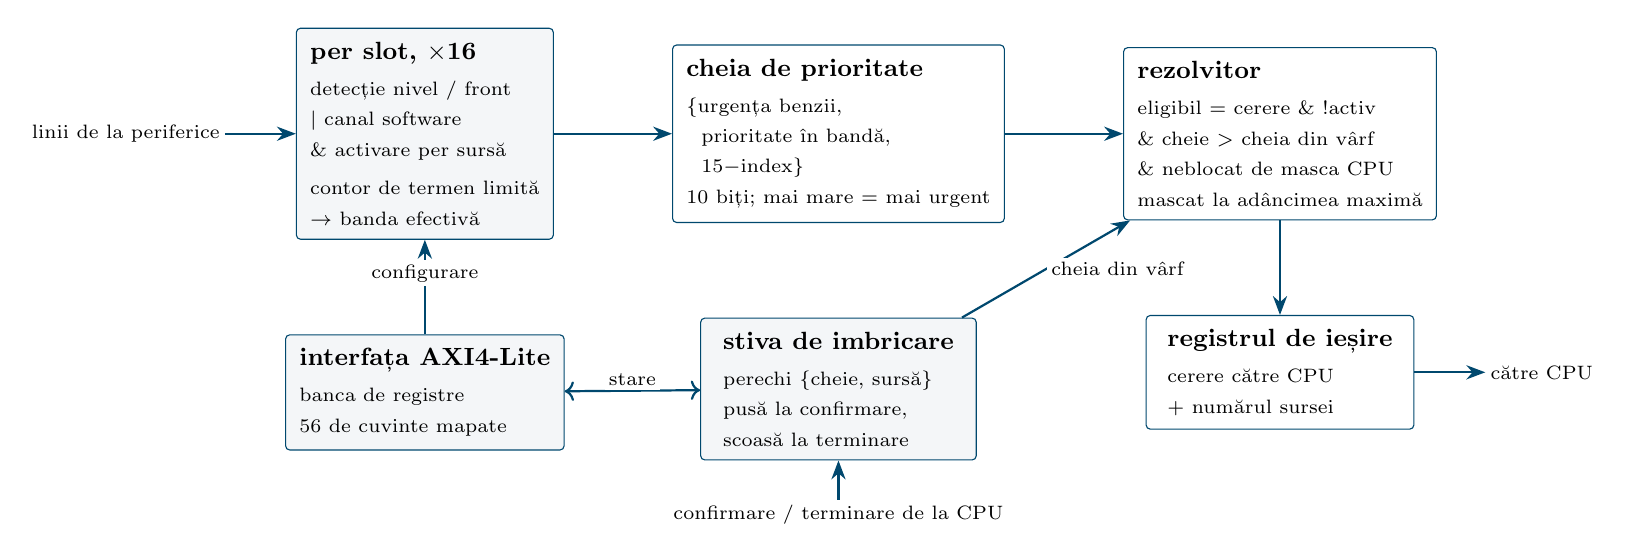
\begin{tikzpicture}[node distance=6mm]
  \node[blkf,minimum width=32mm,align=left] (slot)
    {\textbf{per slot, $\times$16}\\[2pt]
     \scriptsize detecție nivel / front\\
     \scriptsize $\vert$ canal software\\
     \scriptsize \& activare per sursă\\[3pt]
     \scriptsize contor de termen limită\\
     \scriptsize $\to$ banda efectivă};

  \node[blk,right=15mm of slot,minimum width=35mm,align=left] (key)
    {\textbf{cheia de prioritate}\\[2pt]
     \scriptsize \{urgența benzii,\\
     \scriptsize \ \ prioritate în bandă,\\
     \scriptsize \ \ $15-$index\}\\
     \scriptsize 10 biți; mai mare = mai urgent};

  \node[blk,right=15mm of key,minimum width=34mm,align=left] (res)
    {\textbf{rezolvitor}\\[2pt]
     \scriptsize eligibil = cerere \& !activ\\
     \scriptsize \& cheie $>$ cheia din vârf\\
     \scriptsize \& neblocat de masca CPU\\
     \scriptsize mascat la adâncimea maximă};

  \node[blk,below=12mm of res,minimum width=34mm,align=left] (reg)
    {\textbf{registrul de ieșire}\\[2pt]
     \scriptsize cerere către CPU\\
     \scriptsize $+$ numărul sursei};

  \node[blkf,below=12mm of key,minimum width=35mm,align=left] (stack)
    {\textbf{stiva de imbricare}\\[2pt]
     \scriptsize perechi \{cheie, sursă\}\\
     \scriptsize pusă la confirmare,\\
     \scriptsize scoasă la terminare};

  \node[blkf,below=12mm of slot,minimum width=32mm,align=left] (axi)
    {\textbf{interfața AXI4-Lite}\\[2pt]
     \scriptsize banca de registre\\
     \scriptsize 56 de cuvinte mapate};

  \draw[flow] (slot) -- (key);
  \draw[flow] (key) -- (res);
  \draw[flow] (res) -- (reg);
  \draw[flow] (stack) -- node[lbl,right]{cheia din vârf} (res);
  \draw[flow] (axi) -- node[lbl,above]{configurare} (slot);
  \draw[flow,<->] (axi) -- node[lbl,above]{stare} (stack);
  \draw[flow] (reg.east) -- ++(9mm,0) node[lbl,right,align=left]{\scriptsize către CPU};
  \draw[flow] ($(stack.south)+(0,-1mm)$) ++(0,-4mm) -- (stack.south)
        node[lbl,below=5mm,align=center]{\scriptsize confirmare / terminare de la CPU};
  \draw[flow] (slot.west) ++(-9mm,0) -- (slot.west)
        node[lbl,left=9mm]{\scriptsize linii de la periferice};
\end{tikzpicture}}
\caption{Structura internă a controlerului de întreruperi. Rezolvitorul este în
întregime combinațional; singurul etaj înregistrat pe calea cererii este
perechea de ieșire. Am ales asta ca latența de la apariția unei surse la oferta
către procesor să fie de exact un ciclu, indiferent câte surse concurează.}
\label{fig:picblock}
\end{figure}

\section{Cum este aleasă o cerere}

Rezoluția se face pe o \textbf{cheie de prioritate} de 10 biți, construită din
trei câmpuri concatenate. Comparația între două surse devine astfel o simplă
comparație de numere întregi, ceea ce înseamnă un singur comparator în loc de o
cascadă de reguli:

\begin{table}[H]
\centering
\caption{Câmpurile cheii de prioritate, de la cel mai semnificativ}
\label{tab:key}
\small
\begin{tabular}{@{}lcL{0.55\linewidth}@{}}
\toprule
\textbf{Câmp} & \textbf{Biți} & \textbf{Rol} \\
\midrule
Urgența benzii & 2 &
  Sursele sunt grupate în patru benzi; ordinea benzilor este programabilă, deci
  software-ul poate rearanja urgențele fără să reconfigureze fiecare sursă. \\
Prioritate în bandă & 4 &
  Ordonează sursele din aceeași bandă. \\
$15-$index & 4 &
  Departajare finală, deterministă: la egalitate perfectă câștigă sursa cu
  numărul mai mic. Nu există niciodată ambiguitate. \\
\bottomrule
\end{tabular}
\end{table}

O sursă este eligibilă dacă are o cerere activă, nu este deja în tratare, nu
este mascată de procesor, cheia ei este strict mai mare decât cheia din vârful
stivei de imbricare, iar adâncimea stivei nu a atins limita. Ultimele două
condiții sunt exact ceea ce implementează \textbf{preempția}: o sursă mai
urgentă poate întrerupe rutina uneia mai puțin urgente, dar una la fel de
urgentă sau mai puțin urgentă nu.

\section{Ciclul de viață al unei surse}

Controlerul nu are un registru de stare per sursă. Comportamentul de mai jos
este produs de câteva vectoare de indicatoare independente --- front reținut,
cerere software, în tratare, escaladat, spurious. O sursă poate fi deci simultan
în așteptare și escaladată.

\begin{figure}[H]
\centering
\resizebox{\linewidth}{!}{%
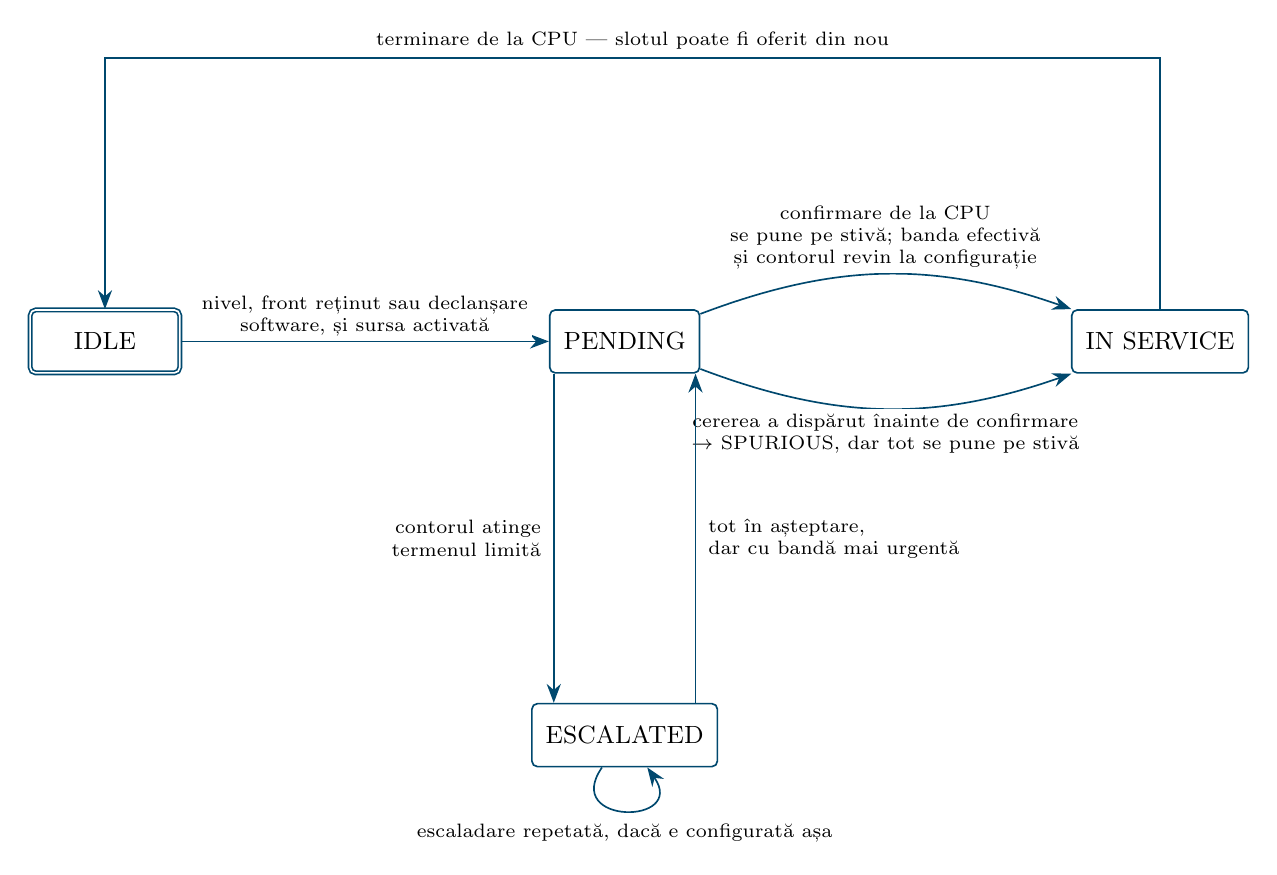
\begin{tikzpicture}[x=1mm,y=1mm,>={Stealth[length=2.4mm]},semithick]
  \node[stbi] (idle) at (0,22)   {IDLE};
  \node[stb]  (pend) at (66,22)  {PENDING};
  \node[stb]  (act)  at (134,22) {IN SERVICE};
  \node[stb]  (esc)  at (66,-28) {ESCALATED};

  \draw[->,draw=accent] (idle) -- node[lbl,above,align=center]
    {nivel, front reținut sau declanșare\\\scriptsize software, și sursa activată} (pend);

  \draw[->,draw=accent] (pend) to[bend left=20]
    node[lbl,above,align=center,pos=0.5]{confirmare de la CPU\\
     \scriptsize se pune pe stivă; banda efectivă\\
     \scriptsize și contorul revin la configurație} (act);
  \draw[->,draw=accent] (pend) to[bend right=20]
    node[lbl,below,align=center,pos=0.5]
    {cererea a dispărut înainte de confirmare\\\scriptsize $\to$ SPURIOUS, dar tot se pune pe stivă} (act);

  \draw[->,draw=accent] (act.north) -- (134,58) -- (0,58) -- (idle.north);
  \node[lbl,above=0.5mm,align=center] at (67,58)
    {terminare de la CPU --- slotul poate fi oferit din nou};

  \draw[->,draw=accent] ($(pend.south)+(-9,0)$) -- ($(esc.north)+(-9,0)$)
    node[lbl,midway,left=1mm,align=right]{contorul atinge\\\scriptsize termenul limită};
  \draw[->,draw=accent] ($(esc.north)+(9,0)$) -- ($(pend.south)+(9,0)$)
    node[lbl,midway,right=1mm,align=left]{tot în așteptare,\\\scriptsize dar cu bandă mai urgentă};

  \draw[->,draw=accent] (esc) to[out=-125,in=-55,looseness=4]
    node[lbl,below=1mm,align=center]{escaladare repetată, dacă e configurată așa} (esc);
\end{tikzpicture}}
\caption{Ciclul de viață al unei surse. Escaladarea modifică doar banda efectivă
folosită la construirea cheii de prioritate și este anulată la confirmare, nu la
terminare --- din momentul în care sursa a fost preluată, nu mai are sens să fie
grăbită.}
\label{fig:picsrcfsm}
\end{figure}

\subsection{Trei mecanisme care nu sunt evidente}

\paragraph{Cererile spurious.} O sursă declanșată pe nivel poate să dispară
între momentul în care controlerul o oferă și momentul în care procesorul o
confirmă --- perifericul și-a rezolvat singur condiția între timp. Controlerul
tot împinge nivelul pe stivă și tot îl marchează, pentru că procesorul a intrat
deja în rutina de tratare și \emph{trebuie} să iasă din ea printr-un semnal de
terminare. Alternativa --- să nu împingi nimic --- ar lăsa stiva desincronizată
față de nucleu, iar asta este mult mai rău decât o rutină care rulează degeaba
o dată.

\paragraph{Termenele limită și escaladarea.} Fiecare sursă are un contor care
măsoară de cât timp așteaptă neservită. La depășirea unui prag configurabil,
banda ei efectivă urcă, deci cheia ei crește și devine mai probabil să fie
aleasă. Este un mecanism împotriva înfometării: o sursă cu prioritate mică nu
poate fi ignorată la nesfârșit de un flux constant de surse mai urgente.
Contorul este citibil oricând, ceea ce îl face și o măsurătoare de latență per
sursă.

\paragraph{Declanșarea software protejată prin cheie.} Ridicarea unei cereri
software cere scrierea simultană a bitului de cerere \emph{și} a unei chei fixe
în aceeași tranzacție. Ștergerea nu cere cheie. Asimetria este intenționată:
cheia apără împotriva creării accidentale a unei întreruperi, nu împotriva
înlăturării ei.

\section{Harta de registre}

\begin{table}[H]
\centering
\caption{Harta de registre a controlerului de întreruperi, 56 de cuvinte mapate}
\label{tab:picmap}
\small
\begin{tabular}{@{}llllL{0.30\linewidth}@{}}
\toprule
\textbf{Ofset} & \textbf{Registru} & \textbf{Acces} & \textbf{Reset} & \textbf{Rol} \\
\midrule
\texttt{0x00--0x3C} & configurare surse & RW & 0 & Tip de declanșare, bandă, prioritate în bandă, termen limită. \\
\texttt{0x40--0x7C} & declanșare software & RW & 0 & Cerere software, protejată prin cheie. \\
\texttt{0x80--0xBC} & stare surse & RO & 0 & Starea vie a fiecărei surse. \\
\texttt{0xC0} & configurarea benzilor & RW & \texttt{0x1B} & Urgența fiecărei benzi. \\
\texttt{0xC4} & starea imbricării & RO & 0 & Adâncime, sursa din vârf, depășire. \\
\texttt{0xC8} & adâncime maximă & RW & 8 & Limita de imbricare. \\
\texttt{0xCC} & sursa în tratare & RO & 0 & Cea mai interioară sursă activă. \\
\texttt{0xD0} & jurnal spurious & R/W1C & 0 & Jurnal persistent per sursă. \\
\texttt{0xD4} & politica de escaladare & RW & 0 & Cum urcă banda la depășirea termenului. \\
\texttt{0xD8} & activare per sursă & RW & 0 & Masca principală. \\
\texttt{0xDC} & stare globală & R/W1C & 0 & Indicatori persistenți de eveniment. \\
\bottomrule
\end{tabular}
\end{table}

Două decizii din tabelul de mai sus le-am luat explicit și le-am verificat cu
teste dedicate:

\paragraph{Biții rezervați sunt legați hardware la zero.} Orice poziție marcată
rezervată citește 0 și înghite o scriere: valoarea este mascată \emph{înainte}
să ajungă în registru, nu stocată și citită înapoi. Este comportamentul pe care
specificația privilegiată RISC-V îl folosește în aceeași situație, și este ceea
ce permite unei revizii ulterioare să definească unul dintre acei biți fără să
strice software-ul care s-a întâmplat să scrie 1 acolo.

\paragraph{Blocul iese din reset complet dezarmat.} Masca principală este zero,
deci nimic nu poate ajunge la procesor până când software-ul nu înscrie explicit
o sursă. Toate sursele sunt pe nivel, în banda 0, cu prioritate 0 și fără
termene limită. Singurele două registre care nu se resetează la zero sunt cele
unde zero ar fi greșit: ordinea benzilor are nevoie de o ordonare implicită
rezonabilă, iar adâncimea maximă de imbricare de zero ar însemna un controler
care nu oferă niciodată nimic.

\chapter{Integrarea într-un System-on-Chip complet}
\label{ch:integrare}

Cele trei blocuri existau, fiecare trecându-și propriile teste, pe ramuri
separate. Între ele nu exista nimic. Ca să devină un sistem, am scris patru
module noi, un nivel de vârf și o hartă de adrese.

\section{De ce nu ajungea o magistrală obișnuită}
\label{sec:punte}

Prima constatare, și cea care a dictat tot restul, a fost că blocurile nu
vorbesc același protocol.

Motorul DMA este master \textbf{AXI4-Full} și emite rafale \sig{INCR} de opt
cuvinte de 32 de biți. Toate slave-urile din sistem --- memoriile, memoria
duală, perifericele --- sunt \textbf{AXI4-Lite}, care nu are rafale deloc: o
adresă, un cuvânt, un răspuns. Nu există niciun fel de cablare care să le lege.

Am scris deci o punte de protocol, care este slave pe partea dinspre DMA și
master pe partea dinspre magistrală. Ea desface fiecare rafală într-o tranzacție
AXI4-Lite per cuvânt și reconstruiește ceea ce partea Full așteaptă înapoi:
marcajul ultimului cuvânt la citire și \emph{un singur} răspuns pentru toată
rafala la scriere.

\subsection{Calea de citire}

Citirile și scrierile sunt independente, așa cum le ține și AXI, iar fiecare
parte tratează câte o rafală o dată --- atât are masterul DMA în curs simultan.

\begin{figure}[H]
\centering
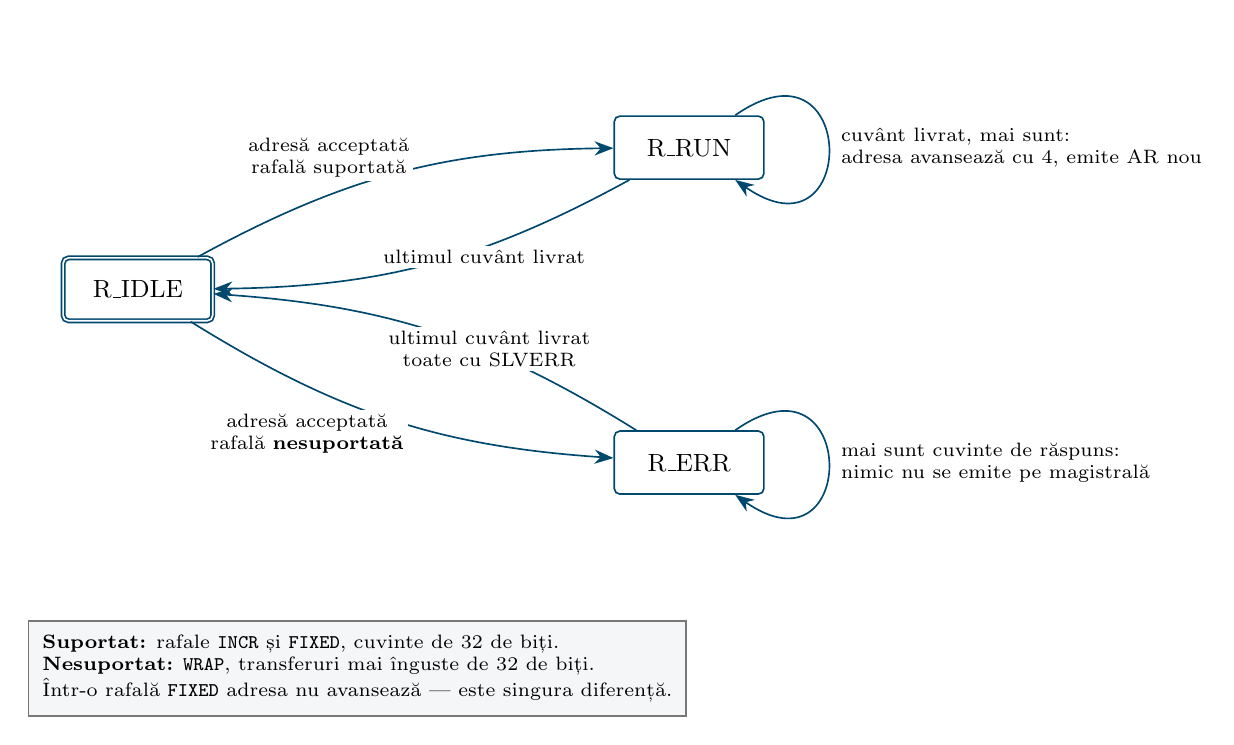
\begin{tikzpicture}[x=1mm,y=1mm,>={Stealth[length=2.4mm]},semithick]
  \node[stbi] (idle) at (0,0)   {R\_IDLE};
  \node[stb]  (run)  at (70,18) {R\_RUN};
  \node[stb]  (err)  at (70,-22){R\_ERR};

  \draw[->,draw=accent] (idle) to[bend left=14]
    node[lbl,pos=0.42,above left=0mm and -6mm,align=center]
    {adresă acceptată\\\scriptsize rafală suportată} (run);
  \draw[->,draw=accent] (idle) to[bend right=14]
    node[lbl,pos=0.42,below left=0mm and -6mm,align=center]
    {adresă acceptată\\\scriptsize rafală \textbf{nesuportată}} (err);

  \draw[->,draw=accent] (run) to[bend left=14]
    node[lbl,pos=0.55,above right=0mm and -4mm,align=center]
    {ultimul cuvânt livrat} (idle);
  \draw[->,draw=accent] (err) to[bend right=14]
    node[lbl,pos=0.55,below right=0mm and -4mm,align=center]
    {ultimul cuvânt livrat\\\scriptsize toate cu SLVERR} (idle);

  \draw[->,draw=accent] (run) to[out=35,in=-35,looseness=6]
    node[lbl,right=1mm,align=left]{\scriptsize cuvânt livrat, mai sunt:
      \\\scriptsize adresa avansează cu 4, emite AR nou} (run);
  \draw[->,draw=accent] (err) to[out=35,in=-35,looseness=6]
    node[lbl,right=1mm,align=left]{\scriptsize mai sunt cuvinte de răspuns:
      \\\scriptsize nimic nu se emite pe magistrală} (err);

  \node[align=left,font=\scriptsize,anchor=north west,
        draw=rulegrey,fill=boxbg,inner sep=5pt] at (-14,-42)
    {\textbf{Suportat:} rafale \sig{INCR} și \sig{FIXED}, cuvinte de 32 de biți.\\
     \textbf{Nesuportat:} \sig{WRAP}, transferuri mai înguste de 32 de biți.\\
     Într-o rafală \sig{FIXED} adresa nu avansează --- este singura diferență.};
\end{tikzpicture}
\caption{Mașina de stări a căii de citire din punte. Starea de eroare există ca
să răspundă la o rafală nesuportată \emph{fără} să emită nimic pe magistrală.}
\label{fig:brgread}
\end{figure}

Calea de date la citire este o trecere directă, nu o memorare urmată de
retransmitere: cuvântul venit de pe partea Lite comandă direct canalul de date
al părții Full, iar disponibilitatea masterului condiționează disponibilitatea
punții. Am ales așa pentru că menține latența la un ciclu în loc de două, și nu
poate nici să reordoneze, nici să piardă date --- nu există niciun tampon în
care ceva să rămână.

\subsection{Calea de scriere și răspunsul persistent}

Scrierea are o diferență esențială față de citire: AXI4-Full dă unei rafale
\textbf{exact un} răspuns de scriere, în timp ce puntea primește câte unul de la
fiecare dintre cele opt tranzacții Lite. Trebuie deci să le combine.

\begin{figure}[H]
\centering
\resizebox{\linewidth}{!}{%
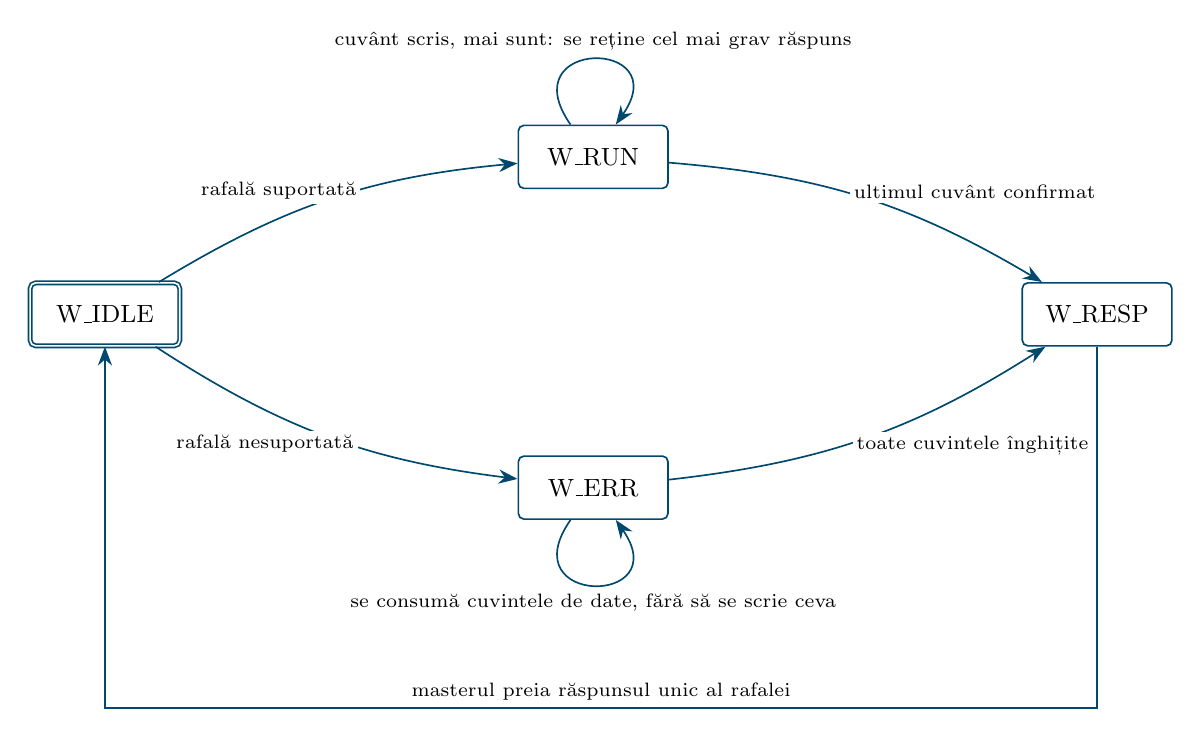
\begin{tikzpicture}[x=1mm,y=1mm,>={Stealth[length=2.4mm]},semithick]
  \node[stbi] (idle) at (0,0)    {W\_IDLE};
  \node[stb]  (run)  at (62,20)  {W\_RUN};
  \node[stb]  (err)  at (62,-22) {W\_ERR};
  \node[stb]  (resp) at (126,0)  {W\_RESP};

  \draw[->,draw=accent] (idle) to[bend left=13]
    node[lbl,pos=0.45,above left=0mm and -6mm,align=center]{rafală suportată} (run);
  \draw[->,draw=accent] (idle) to[bend right=13]
    node[lbl,pos=0.45,below left=0mm and -6mm,align=center]{rafală nesuportată} (err);

  \draw[->,draw=accent] (run) to[bend left=13]
    node[lbl,pos=0.55,above right=0mm and -4mm,align=center]
    {ultimul cuvânt confirmat} (resp);
  \draw[->,draw=accent] (err) to[bend right=13]
    node[lbl,pos=0.55,below right=0mm and -4mm,align=center]
    {toate cuvintele înghițite} (resp);

  % întoarcerea trece pe sub tot, ca să nu atingă bucla lui W\_ERR
  \draw[->,draw=accent] (resp.south) -- (126,-50) -- (0,-50) -- (idle.south);
  \node[lbl,above=0.4mm] at (63,-50) {masterul preia răspunsul unic al rafalei};

  \draw[->,draw=accent] (run) to[out=125,in=55,looseness=6]
    node[lbl,above=0.5mm,align=center]
    {\scriptsize cuvânt scris, mai sunt: se reține cel mai grav răspuns} (run);
  \draw[->,draw=accent] (err) to[out=-125,in=-55,looseness=6]
    node[lbl,below=0.5mm,align=center]
    {\scriptsize se consumă cuvintele de date, fără să se scrie ceva} (err);
\end{tikzpicture}}
\caption{Mașina de stări a căii de scriere. Starea finală există exact pentru că
protocolul cere un singur răspuns pe rafală: el nu poate fi trimis până nu s-a
încheiat ultima tranzacție Lite.}
\label{fig:brgwrite}
\end{figure}

Am luat două decizii aici, și pe amândouă le consider printre cele mai
importante din tot proiectul:

\begin{itemize}[itemsep=4pt,topsep=3pt]
\item \textbf{Răspunsul rafalei este cel mai grav răspuns primit de oricare
      cuvânt din ea.} Dacă al treilea cuvânt din opt eșuează, iar restul reușesc,
      rafala raportează eroare. Alternativa --- să raportezi ultimul răspuns ---
      ar face ca un transfer parțial eșuat să arate curat, ceea ce este exact
      tipul de defect care se descoperă abia în producție.
\item \textbf{O rafală nesuportată nu este tradusă greșit, ci refuzată.} O
      rafală de tip \sig{WRAP} sau un transfer mai îngust primește \sig{SLVERR}
      pe toată lungimea ei, iar pe magistrală nu se emite absolut nimic. A
      transforma în tăcere o rafală neînțeleasă în adrese greșite este felul în
      care o punte corupe memoria într-un mod pe care nimeni nu-l găsește o
      săptămână.
\end{itemize}

\begin{nota}
Puntea răspunde la rafala nesuportată \emph{integral}: îi datorează masterului
tot atâtea cuvinte câte a cerut, doar că fiecare vine cu eroare. Dacă ar
răspunde mai puține, masterul ar rămâne blocat așteptând restul --- iar un
master blocat este mult mai greu de diagnosticat decât un transfer care a
eșuat curat.
\end{nota}

\section{Decodorul de adrese și bucla combinațională}
\label{sec:decodor}

Decodorul rutează un master către unul dintre $N$ slave-uri, în funcție de
adresă, și răspunde el însuși cu \sig{DECERR} la orice adresă care nu cade în
nicio fereastră. Fără acest răspuns propriu, un acces nemapat ar bloca masterul
la nesfârșit, așteptând un răspuns care nu vine niciodată --- cel mai derutant
mod în care poate eșua o magistrală.

Cea mai importantă decizie din decodor este că cele două faze ale unei
tranzacții nu sunt rutate după același criteriu.

\begin{atentie}
\textbf{Faza de adresă și faza de răspuns nu se rutează la fel.} Faza de adresă
este rutată după adresa vie de pe magistrală, cât timp semnalul ei de validare
este sus, astfel încât datele de scriere prezentate odată cu adresa să urmeze
același slave. Faza de răspuns este rutată \textbf{exclusiv} după selecția
memorată la handshake-ul de adresă --- niciodată după adresa vie.

Motivul este că altfel se închide o buclă combinațională prin decodor. Unitatea
de fetch a instrucțiunilor emite adresa pentru instrucțiunea $N+1$ \emph{în
același ciclu} în care primește datele pentru instrucțiunea $N$. Dacă
multiplexorul de răspuns s-ar uita la adresa vie, validitatea datelor citite ar
depinde combinațional de validitatea adresei; iar cum validitatea adresei depinde
de cuvântul tocmai primit, cele două s-ar închide în buclă, iar simularea s-ar
opri cu o eroare de limită de iterații.

Selecția memorată nu este doar o ocolire a buclei, ci este și corectă pe fond: un
răspuns nu poate apărea decât după handshake-ul propriei adrese, deci în momentul
în care răspunsul poate exista, selecția memorată este întotdeauna cea potrivită.
\end{atentie}

\begin{figure}[H]
\centering
\resizebox{\linewidth}{!}{%
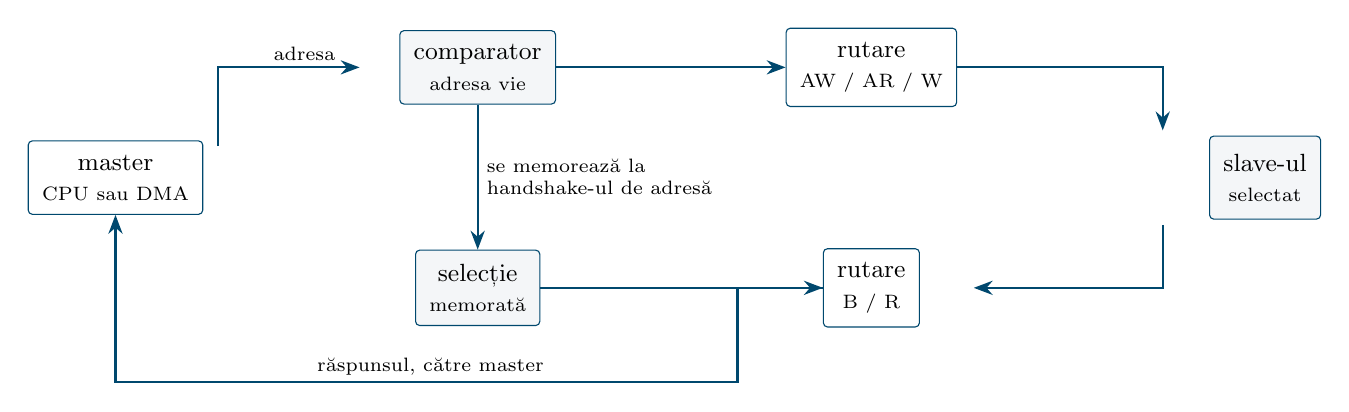
\begin{tikzpicture}[x=1mm,y=1mm,font=\small]
  \node[blk,minimum width=26,minimum height=13] (m) at (0,0)
        {master\\\scriptsize CPU sau DMA};
  \node[blkf,minimum width=30,minimum height=13] (cmp) at (46,14)
        {comparator\\\scriptsize adresa vie};
  \node[blkf,minimum width=30,minimum height=13] (lat) at (46,-14)
        {selecție\\\scriptsize memorată};
  \node[blk,minimum width=26,minimum height=13] (mux1) at (96,14)
        {rutare\\\scriptsize AW / AR / W};
  \node[blk,minimum width=26,minimum height=13] (mux2) at (96,-14)
        {rutare\\\scriptsize B / R};
  \node[blkf,minimum width=26,minimum height=30] (sl) at (146,0)
        {slave-ul\\\scriptsize selectat};

  \draw[flow] (13,4)  -- (13,14) -- (31,14);
  \draw[flow] (cmp)   -- (mux1);
  \draw[flow] (mux1)  -- (133,14) -- (133,6);
  \node[lbl,above=0.3mm] at (24,14) {adresa};

  \draw[flow] (cmp.south) -- node[lbl,right=0.5mm,align=left]
        {\scriptsize se memorează la\\\scriptsize handshake-ul de adresă} (lat.north);
  \draw[flow] (lat) -- (mux2);
  \draw[flow] (133,-6) -- (133,-14) -- (109,-14);
  \draw[flow] (mux2.west) -- (79,-14) -- (79,-26) -- (0,-26) -- (m.south);
  \node[lbl,above=0.3mm] at (40,-26) {răspunsul, către master};

\end{tikzpicture}}
\caption{Cele două căi de rutare din decodor. Faza de adresă urmează adresa vie;
faza de răspuns urmează exclusiv selecția memorată la handshake-ul de adresă.}
\label{fig:decroute}
\end{figure}

Un al doilea detaliu, mai mic dar din aceeași familie: comparațiile de adresă
sunt condiționate de validitatea adresei. Magistrala de adrese a unui master
este nedefinită între tranzacții, fiindcă registrele de sarcină utilă nu au
reset. O comparație necondiționată ar propaga valori nedefinite în
multiplexoarele de disponibilitate, iar valorile nedefinite se propagă tăcut
prin tot sistemul.

\section{Arbitrul}

Unde doi masteri trebuie să împartă un slave cu un singur port --- în sistemul
de față, portul de date al procesorului și DMA-ul, pe memoria de date --- am
pus un arbitru round-robin.

\begin{figure}[H]
\centering
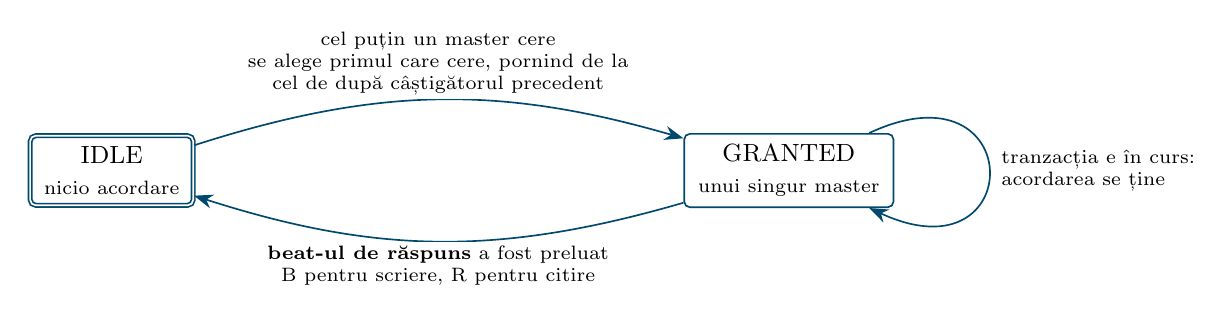
\begin{tikzpicture}[x=1mm,y=1mm,>={Stealth[length=2.4mm]},semithick]
  \node[stbi] (idle) at (0,0)  {IDLE\\\scriptsize nicio acordare};
  \node[stb]  (busy) at (86,0) {GRANTED\\\scriptsize unui singur master};

  \draw[->,draw=accent] (idle) to[bend left=17]
    node[lbl,pos=0.5,above,align=center]
    {cel puțin un master cere\\
     \scriptsize se alege primul care cere, pornind de la\\
     \scriptsize cel de după câștigătorul precedent} (busy);

  \draw[->,draw=accent] (busy) to[bend left=17]
    node[lbl,pos=0.5,below,align=center]
    {\textbf{beat-ul de răspuns} a fost preluat\\
     \scriptsize B pentru scriere, R pentru citire} (idle);

  \draw[->,draw=accent] (busy) to[out=25,in=-25,looseness=6]
    node[lbl,right=1mm,align=left]
    {\scriptsize tranzacția e în curs:\\\scriptsize acordarea se ține} (busy);
\end{tikzpicture}
\caption{Arbitrul. O acordare durează exact o tranzacție și este eliberată pe
beat-ul de răspuns, nu la handshake-ul de adresă.}
\label{fig:arbfsm}
\end{figure}

Momentul eliberării acordării este singura decizie reală aici, și este ușor de
greșit. Dacă acordarea s-ar elibera la handshake-ul de \emph{adresă}, al doilea
master ar putea primi slave-ul în timp ce răspunsul primului este încă pe drum,
iar acel răspuns ar ajunge la masterul greșit. Ținând acordarea până la beat-ul
de răspuns, o tranzacție este indivizibilă.

Pornirea căutării de la masterul de după ultimul câștigător este ceea ce face
arbitrul round-robin în loc de prioritate fixă --- și, cum o acordare durează o
singură tranzacție AXI4-Lite (care nu are rafale), niciun master nu poate ține
slave-ul un timp nelimitat și niciunul nu poate fi înfometat.

Un master care nu are acordarea își vede pur și simplu semnalele de
disponibilitate joase, ceea ce protocolul permite pe termen nedefinit. Nu vede
niciodată un handshake parțial, pentru că numai semnalele masterului acordat
sunt conectate la slave.

\section{Memoriile și nivelul de vârf}

Am scris și o memorie AXI4-Lite sintetizabilă, cu măști pe octet și încărcare de
imagine la pornire, folosită pentru memoria de instrucțiuni și cea de date.
Rațiunea este că sistemul trebuie să fie un proiect complet, nu unul care se
elaborează doar cu un model comportamental atașat. Matricea este ștearsă înainte
de încărcarea imaginii, deci nicio valoare nedefinită nu ajunge la procesor.

Memoria are și parametri de latență și de contra-presiune, inerți la valorile
implicite. Ei sunt cei care permit regresiei să parcurgă temporizări diferite de
magistrală --- vezi Secțiunea~\ref{sec:sweep}.

Nivelul de vârf leagă totul: procesorul, motorul DMA, memoria duală, cele două
memorii, controlerul de întreruperi, temporizatorul, cele trei decodoare,
arbitrul și puntea. Harta de adrese este definită într-un singur loc și dată ca
parametru fiecărui decodor, deci nu există nicio adresă scrisă de mână în
sistem.

\section{Delimitarea față de blocurile colegilor}

Integrarea respectă o regulă explicită: \textbf{nicio schimbare de algoritm în
blocul altcuiva}. Nicio mașină de stări, nicio arbitrare și niciun detector de
coliziuni din blocurile colegilor nu este modificat de magistrala pe care am
scris-o.

\begin{table}[H]
\centering
\caption{Ce atinge integrarea, în funcție de cine deține codul}
\label{tab:integr-schimbari}
\small
\begin{tabular}{@{}L{0.26\linewidth}L{0.64\linewidth}@{}}
\toprule
\textbf{Cine deține codul} & \textbf{Ce face integrarea} \\
\midrule
Blocul propriu: procesor, controler de întreruperi, temporizator, harta de
adrese &
  Îl modific direct. Proprietățile pe care regresia le fixează
  peste ele sunt în Secțiunea~\ref{sec:defecte}. \\
\addlinespace
Blocurile colegilor: motorul DMA, memoria duală &
  Nu le ating. Ce este găsit acolo se documentează cu fișier și linie și se trimite
  proprietarului, care decide. A repara codul altcuiva în ramura de integrare ar
  face ca versiunea lui și a mea să divergă tăcut, iar testele lui ar continua să
  ruleze pe cod care nu mai este cel livrat. \\
\addlinespace
Nici numele porturilor lor &
  Convenția de denumire diferă între blocuri, dar rescrierea listei de porturi a
  unui bloc îi schimbă interfața și îi invalidează testbench-urile
  proprii; nivelul de vârf se conectează la numele așa cum sunt. \\
\bottomrule
\end{tabular}
\end{table}

\section{Traseul complet, pas cu pas}

Ce se întâmplă efectiv când software-ul cere un transfer --- scenariul din tema
stagiului, urmărit prin tot ce am scris:

\begin{enumerate}[itemsep=2pt,topsep=3pt]
\item Programul construiește un descriptor în memoria de date: sursă,
      destinație, lungime, control.
\item Scrie adresa descriptorului și bitul de pornire în registrele DMA-ului,
      pe portul de date al procesorului, prin decodorul de date, ieșirea 4.
\item Activează sursa în controlerul de întreruperi și bitul din registrul de
      activare al procesorului, apoi execută instrucțiunea de așteptare;
      magistrala de instrucțiuni tace.
\item Canalul DMA își aduce descriptorul și emite rafale. Fiecare rafală intră
      în punte, care o desface în opt tranzacții AXI4-Lite.
\item Fiecare tranzacție intră în decodorul DMA-ului: cele către memoria de date
      se așază la coadă în arbitru, alături de cererile procesorului; cele către
      memoria duală merg direct la portul B.
\item La terminare, canalul își ridică linia de întrerupere; ea trece prin masca
      DMA-ului, prin cea a controlerului, și ajunge la procesor.
\item Procesorul se trezește, confirmă preluarea, execută rutina de tratare,
      compară ce a mutat DMA-ul cu ce i-a cerut, și anunță terminarea.
\end{enumerate}

% ===========================================================================
\chapter{Verificarea}
\label{ch:verificare}

Jumătate din titlul temei este „verificare avansată”, și aproape jumătate din
timpul stagiului a mers acolo.

\section{Strategia}

Am folosit patru mecanisme diferite, pentru că fiecare vede altceva:

\begin{table}[H]
\centering
\caption{Cele patru mecanisme de verificare și ce vede fiecare}
\label{tab:verifstrat}
\small
\begin{tabular}{@{}L{0.23\linewidth}L{0.67\linewidth}@{}}
\toprule
\textbf{Mecanism} & \textbf{Ce vede, și ce nu vede} \\
\midrule
Teste direcționate,\newline auto-verificatoare &
  Verifică scenarii concrete: „scriu asta, aștept atâta, trebuie să citesc
  aceea”. Fiecare test își compară singur rezultatul și tipărește un verdict, deci
  un jurnal poate fi validat numărând verdicte, nu citindu-l. Nu vede însă decât
  scenariile la care m-am gândit. \\
\addlinespace
Aserțiuni &
  Reguli permanente, verificate în fiecare ciclu al fiecărei simulări în care
  sunt active. Ele prind încălcări în situații la care nu s-a gândit nimeni ---
  dar numai încălcări de \emph{regulă}, nu rezultate greșite. \\
\addlinespace
Acoperire funcțională &
  Arată ce a rămas neexersat. Nu spune că ceva e corect; spune că ceva nu a fost
  încercat niciodată. \\
\addlinespace
Regresie &
  Rulează totul dintr-o singură compilare, la fiecare modificare. Rolul ei nu
  este să găsească defecte noi, ci să împiedice reapariția celor vechi. \\
\bottomrule
\end{tabular}
\end{table}

Peste ele am adăugat o a cincea metodă, care s-a dovedit cea mai valoroasă:
\textbf{injectarea deliberată de defecte}, descrisă în
Secțiunea~\ref{sec:mutatii}.

\section{Mediul de verificare}

Testbench-urile de bloc verifică fiecare modul separat: unitatea aritmetică,
predictorul de branch, registrele de control, cauzele de trap, controlerul de
întreruperi cu benzile și imbricarea lui, temporizatorul. Testbench-urile de
sistem verifică ansamblul.

Cele de sistem sunt speciale prin faptul că \textbf{verificarea o face
software-ul, nu testbench-ul}. Testbench-ul furnizează doar un ceas, un reset și
o imagine de memorie; programul asamblat construiește descriptorul, programează
canalul DMA, adoarme pe instrucțiunea de așteptare, este trezit de întreruperea
de terminare și compară ce a mutat DMA-ul cu ce i-a cerut. Este cea mai apropiată
formă de verificare de utilizarea reală a sistemului.

Am adăugat și monitoare de protocol pe fiecare magistrală, care urmăresc
handshake-urile independent de ce cred masterul și slave-ul că se întâmplă.

\section{Regresia}

\begin{table}[H]
\centering
\caption{Regresia procesorului: 15 rulări dintr-o singură compilare}
\label{tab:regcpu}
\small
\begin{tabular}{@{}cL{0.26\linewidth}L{0.46\linewidth}@{}}
\toprule
\textbf{Rulări} & \textbf{Ce verifică} & \textbf{Observație} \\
\midrule
1--4  & Sistem cu un nucleu & Aceleași teste sub patru temporizări diferite de magistrală. \\
5     & Două nuclee, memorie partajată & Handshake între nuclee. \\
6--7  & Controlerul de întreruperi & Funcțional, apoi colțurile de planificare: masca procesorului, frontul sosit exact în ciclul confirmării, escaladarea, declanșarea cu cheie. \\
8--10 & Reset, registre read-only, stare per sursă & Fiecare bit rezervat și fiecare registru numai-citire, individual. \\
11    & Temporizatorul & Registre, armare, rostogolire. \\
12    & Registre de control și stare & Numai-citire, valori inadmisibile, reset. \\
13    & Cauzele de trap & Câte un test dedicat pentru fiecare cauză. \\
14    & Predictorul de branch & Tabel, stivă de retur, limite, reset. \\
15    & Unitatea aritmetică & Decodarea operațiilor și valorile de la limită. \\
\bottomrule
\end{tabular}
\end{table}

\begin{table}[H]
\centering
\caption{Regresia sistemului: 24 de rulări dintr-o singură compilare}
\label{tab:regsoc}
\small
\begin{tabular}{@{}clL{0.52\linewidth}@{}}
\toprule
\textbf{Rulări} & \textbf{Ce verifică} & \textbf{De ce există separat} \\
\midrule
1--2  & Harta de adrese & Întâi cele două declarații ale hărții, una față de alta; apoi ferestrele în circuit. Verifică o proprietate pe care niciun program corect nu o poate atinge: software-ul corect nu emite niciodată o adresă care nu trebuie să decodeze. \\
3--4  & Puntea de protocol & Singura bucată de logică nouă prin care trece toată calea de date a sistemului, testată izolat: întâi rafalele curate, apoi o eroare pe un beat din interiorul rafalei. \\
5     & Perifericele sub contra-presiune & Controlerul, temporizatorul și memoria duală cu răspunsul ținut 1, 3 și 10 cicluri. \\
6--9  & Sistemul complet & Software real pe procesor real, conducând un transfer DMA real, cu procesorul adormit cât timp acesta se desfășoară. \\
10--13& Sistemul sub stres & Același sistem, cu procesorul lucrând pe magistrală tot timpul. Este grupul care atinge logica de contenție. \\
14--17& Lungimi de transfer & Cinci lungimi care nu sunt multipli întregi de rafală: 64, 40, 20, 8 și 4 octeți. \\
18--20& Canalele DMA & O întrerupere mascată la periferic, cele patru canale în arbitrare round-robin, și o rafală care depășește fereastra. \\
21    & Temporizatorul & Armat de un program, cu întreruperea livrată prin controler. \\
22--24& Controlerul, prin procesor & Toate cele șaisprezece surse pe rând, preempția și imbricarea, și escaladarea pe termen limită. \\
\bottomrule
\end{tabular}
\end{table}

Grupul de stres și cel de lungimi există fiindcă am \emph{măsurat} că testul de
sistem simplu nu le atingea:

\begin{itemize}[itemsep=4pt,topsep=3pt]
\item Testul de sistem simplu \textbf{nu a contendat niciodată arbitrul}, nu a
      atins niciodată ambele porturi ale memoriei duale în același ciclu și nu a
      produs nicio coliziune reală. Trecea fără să exerseze nimic din toate
      acestea. Testul de stres le măsoară și \textbf{cade dacă nu s-au
      întâmplat}, deci acoperirea nu poate să se degradeze tăcut.
\item Cele două programe de sistem mută 64 și 256 de octeți --- multipli exacți
      ai rafalei de 32 de octeți. Calea rafalei finale scurte era deci
      inaccesibilă din testele de sistem, iar exact acolo scrie un DMA dincolo de
      ce i s-a cerut. Testul de lungimi citește direct matricea memoriei și cade
      atât la un cuvânt livrat scurt, cât și la unul scris dincolo de capăt.
\end{itemize}

\subsection{Parcurgerea temporizărilor de magistrală}
\label{sec:sweep}

Fiecare test la nivel de sistem rulează sub patru temporizări de magistrală:
nominală, latență fixă mare, și două semințe diferite de contra-presiune
aleatoare pe semnalele de disponibilitate.

Motivul este direct: o magistrală care funcționează numai când fiecare slave
răspunde într-un ciclu nu a fost testată. Decodorul ține o selecție memorată
peste răspuns, arbitrul ține o acordare peste el, iar puntea ține un contor de
cuvinte peste el --- și toate trei sunt exact genul de stare care se strică doar
când slave-ul își ia timp.

Pragurile de acoperire sunt impuse în \emph{toate} cele patru configurații, nu
doar în cea nominală. Nu era garantat: latența injectată schimbă planificarea,
deci programul ajunge de fiecare dată în alte colțuri. Măsurat, pragurile se
țin peste tot --- arbitrul este contendat între 161 și 224 de cicluri, și cel
puțin o coliziune reală de adresă apare în fiecare configurație.

\section{Aserțiunile}
\label{sec:sva}

Stratul de aserțiuni este legat de circuit, nu scris în el, și rulează pe
Verilator, fiindcă ediția de ModelSim disponibilă nu compilează aserțiuni. El
acoperă trei zone: protocolul AXI4-Lite și AXI4-Full pe fiecare port,
invarianții nucleului și ai controlerului de întreruperi, și deciziile proprii
ale magistralei:

\begin{itemize}[itemsep=1pt,topsep=3pt]
\item ferestrele de adresă sunt disjuncte;
\item acordarea arbitrului este one-hot, adică cel mult un master este servit;
\item acordarea este ținută până la beat-ul de răspuns;
\item un master neacordat nu vede niciun handshake;
\item contorul de cuvinte al punții și marcajul de ultim cuvânt sunt de acord;
\item confirmarea și terminarea întreruperii sunt impulsuri de un ciclu și nu
      apar niciodată în același ciclu;
\item adâncimea de imbricare se mișcă numai pe aceste două impulsuri și nu
      trece niciodată de limită.
\end{itemize}

Stratul rulează pe toate cele cincisprezece testbench-uri ale fluxului Verilator
de sistem, plus testul de sistem al procesorului, fără nicio declanșare.

\begin{nota}
\textbf{O aserțiune care nu e legată nu verifică nimic.} Am verificat explicit
că stratul chiar este activ, nu doar prezent: aceeași simulare compilată fără
suportul de aserțiuni raportează zero aserțiuni, iar cu el le raportează pe ale
sale și indică drumul ierarhic din interiorul circuitului. Verificarea pare paranoică,
dar un strat de aserțiuni prezent în surse și nelegat de circuit arată, într-un
jurnal de simulare, exact la fel ca unul care funcționează.
\end{nota}

\section{Injectarea deliberată de defecte}
\label{sec:mutatii}

Un test care trece poate trece din motive greșite până la proba contrarie. Ca să
aflu care este cazul, am injectat șapte defecte, unul câte unul, și am rulat
regresia completă pentru fiecare.

\begin{table}[H]
\centering
\caption{Defecte injectate deliberat și testul care le prinde}
\label{tab:mutatii}
\small
\begin{tabular}{@{}L{0.52\linewidth}L{0.36\linewidth}@{}}
\toprule
\textbf{Defect injectat} & \textbf{Prins de} \\
\midrule
Prioritatea coliziunii din memoria duală, inversată & testul de stres \\
Persistența răspunsului de eroare, eliminată din punte & testul de eroare pe un beat din rafală \\
Fereastra memoriei duale lărgită la de patru ori dimensiunea ei & testul hărții de adrese \\
Acordarea arbitrului eliberată la handshake-ul de adresă & testul de sistem \\
Răspunsul decodorului rutat după adresa vie & bucla combinațională oprește simularea \\
Marcajul de ultim cuvânt mutat cu un cuvânt mai devreme & testul punții, toate testele de sistem, și o aserțiune \\
Masca de întreruperi ignorată la formarea liniei & testul canalului DMA cu întreruperea mascată \\
\bottomrule
\end{tabular}
\end{table}

\textbf{Fiecare dintre cele șapte cade acum în regresie.} Două nu cădeau la
prima rundă de injectare --- persistența răspunsului de eroare și masca de
întreruperi --- și exact acelea două au dat ultimele două testbench-uri: unul care
răspunde cu eroare pe un beat ales din interiorul rafalei, altul care lasă un
canal DMA cu întreruperea mascată. Injectarea nu a găsit un defect în circuit;
a arătat unde suita nu se uita.

Rezultatul este cel mai util al întregului stagiu, pentru că este singurul care
spune ceva despre \emph{suită}, nu despre circuit: un raport de acoperire arată
ce nu a fost atins, iar injectarea unui defect arată dacă ceea ce a fost atins
era și privit.

\section{Proprietăți pe care regresia le fixează explicit}
\label{sec:defecte}

Nouă proprietăți ale blocului meu nu se citesc din structura codului și se pierd
tăcut dacă cineva le atinge: comportamentul rămâne rezonabil în cazul obișnuit și
se rupe într-un colț. Fiecare are un test dedicat în regresie, care cade dacă
proprietatea dispare. Împreună, ele sunt specificația fină a blocului --- partea
pe care o hartă de registre nu o poate exprima.

\begin{table}[H]
\centering
\caption{Proprietăți fixate de câte un test dedicat}
\label{tab:proprietati}
\small
\begin{tabular}{@{}L{0.56\linewidth}L{0.32\linewidth}@{}}
\toprule
\textbf{Proprietate garantată} & \textbf{Unde este fixată} \\
\midrule
Revenirea dintr-un trap știe ce fel de trap închide: câte un bit per nivel
deschis, 16 adânc. & testbench-ul de cauze de trap \\
\addlinespace
O sursă mascată de procesor nu este oferită și nu blochează sursele mai puțin
urgente din spatele ei. & programul de sistem, la parcurgerea canalelor \\
\addlinespace
Registrul de surse în așteptare arată întregul set în așteptare, nu doar sursa
oferită în acel moment. & testbench-ul funcțional al controlerului \\
\addlinespace
Fereastra fiecărui periferic are exact 256 de octeți, cât banca lui de registre,
deci nimic nu aliasează deasupra blocului. & testbench-ul hărții de adrese \\
\addlinespace
Escaladarea urcă în ordinea de urgență configurată a benzilor; nu presupune că
banda 0 este cea mai urgentă. & testbench-ul de planificare \\
\addlinespace
Un front sosit exact în ciclul confirmării nu se pierde: frontul are prioritate
față de confirmare. & testbench-ul de planificare \\
\addlinespace
Declanșarea software cere bitul de cerere și cheia scrise în aceeași tranzacție;
cheia singură nu face nimic. & testbench-ul de planificare \\
\addlinespace
Vectorul de trap nu stochează moduri rezervate: un mod rezervat se citește ca
mod direct. & testbench-ul de registre read-only \\
\addlinespace
O operație atomică pe un contor de performanță se aplică pe valoarea deja
incrementată, deci evenimentul ciclului curent nu se pierde. & testbench-ul de
registre read-only \\
\bottomrule
\end{tabular}
\end{table}

Compunerea celor două măști de întreruperi este singura dintre ele care nu se
poate rezolva în interiorul unui singur bloc.

\subsection{Compunerea celor două măști de întreruperi}
\label{sec:doua-masti}

O sursă trece prin două măști independente înainte să ajungă la o rutină de
tratare: activarea din controlerul de întreruperi și bitul din registrul de
activare al procesorului. Felul în care cele două se compun este o decizie de
proiectare, nu o consecință automată a faptului că amândouă există.

\textbf{Nucleul predă masca lui controlerului}, iar rezolvitorul sare peste
sursele mascate. O sursă mascată rămâne totuși \emph{în așteptare}: apare în
registrul de surse în așteptare și contorul ei de termen limită continuă să
meargă. Doar că nu este oferită nucleului până când masca se ridică.

Aranjamentul opus --- controlerul alege un câștigător fără să știe nimic despre
masca procesorului, iar procesorul aplică masca asupra câștigătorului primit ---
pare echivalent și nu este. O sursă activată în controler dar mascată în
procesor ar fi aleasă și niciodată preluată: rezolvitorul ar rămâne parcat pe ea,
nimic mai puțin urgent nu ar mai fi oferit vreodată, iar o instrucțiune de
așteptare care depinde de o astfel de sursă nu s-ar mai trezi. Cele două măști
n-ar compune o mască mai strictă, ci un blocaj.

Proprietatea este fixată de programul de sistem, care lasă o sursă activată în
controler și mascată în procesor pe toată durata rulării și verifică dacă
sursele din spatele ei sunt totuși servite.

\section{Rezultate măsurate}

Cifrele de mai jos sunt citite din jurnalul regresiei rulate pe versiunea
curentă a proiectului, nu din memorie.

\begin{table}[H]
\centering
\caption{Rezultatele regresiei complete}
\label{tab:rezultate}
\small
\begin{tabular}{@{}lccl@{}}
\toprule
\textbf{Regresie} & \textbf{Rulări} & \textbf{Verificări} & \textbf{Rezultat} \\
\midrule
Procesor, controler de întreruperi, temporizator & 15 & 2\,561 & toate trec \\
Sistemul complet & 24 & 428 & toate trec \\
\midrule
\textbf{Total} & \textbf{39} & \textbf{2\,989} & \textbf{0 eșecuri} \\
\bottomrule
\end{tabular}
\end{table}

Toate cele trei blocuri se compilează într-o singură bibliotecă, fără erori și
fără avertismente. Analiza statică pe al doilea simulator este curată, iar
stratul de aserțiuni trece fără nicio declanșare pe toate testbench-urile de
sistem. Acoperirea funcțională măsurată pe nucleu atinge 88 din cele 92 de
coșuri și trece pragul impus, fiindcă fiecare coș obligatoriu a fost atins.

% ===========================================================================
\chapter{Rezultate și concluzii}
\label{ch:concluzii}

\section{Ce funcționează}

Sistemul face astăzi exact ce cerea tema, verificat automat:
software rulând pe procesorul pe care l-am proiectat construiește un descriptor,
programează un canal DMA, adoarme, este trezit de întreruperea de terminare
trecută prin controlerul de întreruperi pe care l-am proiectat, și verifică
octet cu octet ce a fost mutat. Aceleași verificări trec sub patru temporizări
diferite de magistrală, inclusiv cu contra-presiune aleatoare, și cu procesorul
lucrând pe magistrală în paralel cu transferul.

Contribuția mea, rezumată:

\begin{table}[H]
\centering
\caption{Ce am livrat}
\label{tab:livrat}
\small
\begin{tabular}{@{}L{0.28\linewidth}L{0.62\linewidth}@{}}
\toprule
\textbf{Componentă} & \textbf{Conținut} \\
\midrule
Procesor RV32I &
  Pipeline pe trei stagii cu trap-uri precise, predictor de branch cu stivă de
  retur, unitate load/store cu măști pe octet și excepții precise, două porturi
  master AXI4-Lite, registre de control M-mode, contoare de performanță,
  instrucțiune de așteptare. \\
\addlinespace
Controler de\newline întreruperi &
  16 surse hardware și 16 canale software, benzi de prioritate programabile,
  preempție cu imbricare până la 16 niveluri, detecție de cereri spurious,
  termene limită cu escaladare, 56 de registre mapate. \\
\addlinespace
Temporizator &
  Contor și comparație pe 64 de biți, cu secvență de armare fără declanșare
  falsă. \\
\addlinespace
Magistrala\newline sistemului &
  Punte AXI4-Full $\rightarrow$ AXI4-Lite, decodor de adrese cu răspuns propriu
  la adrese nemapate, arbitru round-robin, memorie AXI4-Lite sintetizabilă,
  nivelul de vârf și harta de adrese. \\
\addlinespace
Verificare &
  39 de rulări de regresie cu 2\,989 de verificări automate, strat de aserțiuni
  pe fiecare magistrală, acoperire funcțională cu praguri impuse, injectare
  deliberată de defecte, integrare continuă. \\
\bottomrule
\end{tabular}
\end{table}

\begin{table}[H]
\centering
\caption{Scara lucrării, numărată în depozit}
\label{tab:scara}
\small
\begin{tabular}{@{}L{0.54\linewidth}rr@{}}
\toprule
 & \textbf{Fișiere} & \textbf{Linii} \\
\midrule
RTL: procesor, controler de întreruperi, temporizator, magistrală & 23 & 4\,844 \\
Testbench-uri proprii, de bloc și de sistem & 32 & 9\,316 \\
Fișiere de aserțiuni & 9 & --- \\
\bottomrule
\end{tabular}
\end{table}

\section{Ce am învățat}

\subsection{Despre proiectare}

AXI mi-a părut simplu până când a trebuit să scriu un master. Diagrama cu cele
cinci canale se învață în zece minute; ce contează de fapt sunt restricțiile, iar
pe acelea le-am descoperit una câte una, în simulare: o cerere ridicată nu mai
poate fi retrasă, nu se poate presupune nicio ordine între canalul de adresă și
cel de date la o scriere, iar o citire pornită nu se poate anula. Ultima are o
consecință pe care nu o anticipasem --- unitatea de fetch a instrucțiunilor are
un mecanism întreg, indicatorul de aruncare, care există numai pentru că
răspunsul unei citiri deja emise trebuie primit și apoi ignorat.

Al doilea lucru pe care îl duc mai departe ține de cum reprezint starea.
Urmărirea nivelurilor de trap părea, la prima vedere, o treabă pentru un singur
bit --- „suntem sau nu într-o întrerupere”. Cu un bit, comportamentul este corect
pentru un nivel deschis, adică exact cazul pe care îl atinge un test scris fără
intenție adversarială, și greșit pentru două. De atunci, pentru fiecare indicator
de stare pe care îl adaug, mă întreb câte niveluri poate avea simultan lucrul pe
care îl descrie.

Cât despre erori, cele două decizii din punte --- răspunsul cel mai grav câștigă,
iar o rafală neînțeleasă este refuzată în loc să fie tradusă --- vin din aceeași
idee: un sistem care raportează un eșec se poate depana, iar unul care îl ascunde,
nu.

\subsection{Despre verificare}

Cel mai mult mi-a schimbat felul de a gândi momentul în care am măsurat acoperirea
pe un test care trecea. Testul de sistem trece impecabil și, luat singur, nu
atinge arbitrul sub contenție, nu atinge ambele porturi ale memoriei duale în
același ciclu și nu produce nicio coliziune --- adică nu exersează niciuna dintre
situațiile pentru care logica aceea este scrisă. De aceea există testul de stres
alături de el.

Mi-au rămas de acolo două obiceiuri. Pragurile de acoperire se impun, nu se
tipăresc: un test care numără contenții și nu cade când ele lipsesc nu verifică
nimic. Și un test care trece merită tratat ca suspect până când i se arată că
poate să cadă --- injectarea deliberată de defecte este cel mai ieftin mod de a
afla asta, și mi-a spus mai multe despre calitatea suitei mele decât orice raport
de acoperire.

\subsection{Despre lucrul în echipă și documentație}

Trei blocuri dezvoltate în paralel de trei oameni nu se integrează dacă interfața
nu este fixată înainte de a începe. Cele trei înțelegeri din prima săptămână ---
un singur protocol, un singur ceas, întreruperile prin controler --- sunt motivul
pentru care integrarea a fost o problemă de zile, nu de săptămâni.

Regula pe care nu o anticipasem este că un defect din blocul altcuiva se
raportează, nu se repară. Am găsit mai multe probleme în blocurile colegilor și
le-am documentat cu fișier și linie, dar le-au corectat ei, pe ramurile lor. Dacă
le-aș fi corectat eu în ramura de integrare, versiunea lor și a mea ar fi divergat
tăcut, iar testele lor ar fi continuat să ruleze pe cod care nu mai era cel
livrat.

Tot de aici vine și ce am învățat despre documentație. Am scris-o în paralel cu
codul și, scriind-o, am observat că unele afirmații descriau intenția de
proiectare, nu comportamentul implementat. Diferența nu este cosmetică: o
documentație care descrie intenția îl trimite pe următorul integrator într-o
presupunere greșită.

\section{Concluzie}

Stagiul a acoperit până acum un ciclu complet de proiectare digitală: de la
citirea unei specificații și transformarea ei într-o arhitectură, prin
implementare RTL și verificare, până la integrarea cu blocuri scrise de altcineva
și documentarea rezultatului.

Partea cea mai formativă nu a fost scrierea procesorului, deși a fost cea mai
mare ca volum, ci integrarea --- locul unde trei bucăți de logică, fiecare
corectă în izolare, trebuie să se potrivească --- și revizuirea propriei lucrări
pornind de la premisa că greșelile sunt acolo. De acolo îmi rămâne o observație
pe care nu o aveam la început: un comportament greșit, dacă are documentată o
cale de a-l ocoli, arată din interior exact ca o decizie de proiectare. Singurul
mod de a le deosebi este să ceri, pentru fiecare, testul care ar cădea dacă
proprietatea s-ar pierde.

% ===========================================================================
\appendix
\chapter{Tehnologii, instrumente și protocoale}
\label{ch:tehnologii}

\section{Limbaje și instrumente}

Am lucrat exclusiv cu instrumente folosite industrial pentru proiectare
digitală. Alegerile nu au fost ale mele --- tema le-a fixat --- dar motivul
pentru care fiecare există în flux merită enunțat, pentru că fluxul întreg este
unul dintre lucrurile pe care le-am învățat în stagiu.

\begin{table}[H]
\centering
\caption{Instrumentele folosite și rolul fiecăruia în flux}
\label{tab:tools}
\small
\begin{tabular}{@{}L{0.23\linewidth}L{0.68\linewidth}@{}}
\toprule
\textbf{Instrument} & \textbf{Rol} \\
\midrule
Verilog--2005 &
  Limbajul de descriere hardware în care este scris tot circuitul. Am folosit
  strict subsetul sintetizabil: fără construcții comportamentale în calea de
  date, un singur bloc \sig{always} pentru fiecare registru, reset asincron pe
  fiecare bistabil. \\
\addlinespace
SystemVerilog\newline Assertions &
  Aserțiuni care descriu reguli permanente ale protocolului --- de exemplu
  „\sig{VALID} nu poate cădea până nu vine \sig{READY}”. Spre deosebire de un
  test, o aserțiune verifică regula în \emph{fiecare} ciclu al \emph{fiecărei}
  simulări în care este activă. \\
\addlinespace
ModelSim și\newline Verilator &
  Simulatorul principal, pe care rulează regresia completă, și al doilea, folosit
  pentru două lucruri pe care primul nu le face în ediția disponibilă: analiză
  statică strictă și compilarea aserțiunilor. Faptul că aceeași sursă trece pe
  două simulatoare diferite este o verificare în sine --- fiecare tolerează alte
  scăpări. \\
\addlinespace
Asamblor propriu,\newline scris în Python &
  Programele de test rulează pe procesorul propriu, deci trebuie asamblate. Am
  scris un asamblor RV32I care produce imaginea de memorie și, în plus, un
  fișier cu adresele etichetelor, ca testbench-ul să poată verifica unde a ajuns
  execuția fără să conțină adrese scrise de mână. \\
\addlinespace
Makefile &
  Un singur punct de intrare pentru fiecare flux: asamblare, regresie pe
  ModelSim, analiză statică și aserțiuni pe Verilator. O comandă, nu o secvență
  de pași ținuți minte. \\
\addlinespace
Git &
  Model pe ramuri: o ramură per bloc, integrarea pe ramura principală, ramurile
  de bloc niciodată rescrise. \\
\addlinespace
Integrare continuă &
  Fluxul de analiză statică, aserțiuni și acoperire rulează automat la fiecare
  modificare împinsă în depozit, pe Verilator, care este liber și poate rula
  într-un mediu automat. \\
\addlinespace
LaTeX &
  Documentația tehnică și acest raport. Diagramele sunt desenate în TikZ, direct
  în sursa documentului, ca să poată fi corectate odată cu circuitul. \\
\bottomrule
\end{tabular}
\end{table}

\section{Magistrala AXI4-Lite}
\label{sec:axilite}

Toate interfețele din sistem, cu o singură excepție, sunt AXI4-Lite. Este
subsetul simplu al standardului AMBA AXI4: un transfer, o adresă, un cuvânt de
date. Nu are rafale, nu are identificatori de tranzacție și nu permite
reordonarea răspunsurilor.

\subsection{Canale}

Un transfer este purtat pe unul dintre cele cinci canale independente. Fiecare
are handshake-ul lui, și niciunul nu blochează alt canal.

\begin{table}[H]
\centering
\caption{Canalele AXI4-Lite și conținutul fiecăruia}
\label{tab:axichan}
\small
\begin{tabular}{@{}clL{0.46\linewidth}@{}}
\toprule
\textbf{Canal} & \textbf{Direcție} & \textbf{Transportă} \\
\midrule
AW & master $\rightarrow$ slave & Adresa de scriere (\sig{AWADDR}) și tipul de protecție (\sig{AWPROT}). \\
W  & master $\rightarrow$ slave & Datele de scris (\sig{WDATA}) și măștile pe octet (\sig{WSTRB}). \\
B  & slave $\rightarrow$ master & Răspunsul la scriere (\sig{BRESP}). \\
AR & master $\rightarrow$ slave & Adresa de citire (\sig{ARADDR}) și tipul de protecție (\sig{ARPROT}). \\
R  & slave $\rightarrow$ master & Datele citite (\sig{RDATA}) și răspunsul la citire (\sig{RRESP}). \\
\bottomrule
\end{tabular}
\end{table}

O citire folosește AR, apoi R. O scriere folosește AW și W --- care sunt canale
separate și pot fi acceptate în orice ordine --- și se încheie cu B. Nu există
niciun semnal „scriere terminată” în afară de răspunsul B, și acesta este
motivul pentru care fiecare cale de scriere pe care am scris-o urmărește AW și W
independent unul de altul.

\subsection{Handshake-ul}

Toate canalele funcționează la fel. Sursa ridică \sig{VALID} când are ceva de
transferat; destinația ridică \sig{READY} când poate primi. \textbf{Transferul
are loc pe frontul de ceas în care ambele sunt sus.} Oricare dintre ele poate
veni primul.

\begin{figure}[H]
\centering
\begin{tikztimingtable}[timing/slope=0,timing/coldist=3pt,xscale=1.5]
  clk    & 12{C} \\
  VALID  & 2L 2H 2L 4H 2L \\
  READY  & 2L 2H 4L 2H 2L \\
  DATE   & 2U 2D{A} 4D{B} 2D{B} 2U \\
  \extracode
  \begin{pgfonlayer}{background}
    \vertlines[help lines]{2,4,6,8,10}
  \end{pgfonlayer}
\end{tikztimingtable}
\caption{Două transferuri pe același canal. Primul (sarcina utilă~A) se încheie
imediat, pentru că ambele părți sunt gata în același ciclu. Al doilea
(sarcina~B) este ținut de sursă încă două cicluri, cât timp destinația nu este
gata; sarcina utilă nu se schimbă pe durata așteptării.}
\label{fig:axihs}
\end{figure}

Din această regulă decurg două obligații, și amândouă sunt verificate automat pe
fiecare magistrală din sistem, de aserțiunile descrise în
Secțiunea~\ref{sec:sva}:

\begin{enumerate}[itemsep=2pt,topsep=3pt]
\item Odată ridicat, \sig{VALID} nu poate cădea până nu a fost acceptat de
      \sig{READY}. Un master care își retrage cererea pentru că s-a răzgândit
      încalcă protocolul.
\item Cât timp \sig{VALID} este sus și neacceptat, sarcina utilă nu se poate
      schimba. Altfel destinația nu ar ști ce a primit.
\end{enumerate}

\subsection{Codurile de răspuns}

\begin{table}[H]
\centering
\caption{Codurile purtate de \sig{RRESP} și \sig{BRESP}}
\label{tab:axiresp}
\small
\begin{tabular}{@{}clL{0.54\linewidth}@{}}
\toprule
\textbf{Cod} & \textbf{Nume} & \textbf{Înțeles în acest sistem} \\
\midrule
\texttt{00} & \sig{OKAY}   & Transferul a reușit. \\
\texttt{10} & \sig{SLVERR} & Adresa a ajuns la un slave, dar slave-ul a refuzat
              cererea: acces nealiniat, rafală nesuportată, sau coliziune
              pierdută pe memoria dual-port. \\
\texttt{11} & \sig{DECERR} & Adresa nu aparține niciunui slave. Îl produce
              decodorul, nu un periferic. \\
\bottomrule
\end{tabular}
\end{table}

Distincția dintre ultimele două contează practic: \sig{SLVERR} înseamnă „am
ajuns unde trebuia, dar cererea era greșită”, iar \sig{DECERR} înseamnă „nu
există nimic la adresa aceea”. În sistemul de față ambele produc o excepție
precisă în procesor, dar cu cauze distincte, deci un program poate spune care
dintre ele s-a întâmplat.

\section{Ce adaugă AXI4-Full}
\label{sec:axifull}

Portul de master al DMA-ului este AXI4-Full. Diferența relevantă pentru acest
proiect este una singură, dar are consecințe pe tot lanțul.

\begin{table}[H]
\centering
\caption{Diferențele dintre AXI4-Full și AXI4-Lite relevante aici}
\label{tab:fullvslite}
\small
\begin{tabular}{@{}L{0.22\linewidth}L{0.30\linewidth}L{0.34\linewidth}@{}}
\toprule
 & \textbf{AXI4-Lite} & \textbf{AXI4-Full} \\
\midrule
Rafale & Nu există. O adresă, un cuvânt. &
  \sig{AWLEN}/\sig{ARLEN} cer până la 256 de cuvinte pentru o singură adresă. \\
\addlinespace
Ultimul cuvânt & Nu are sens. &
  \sig{WLAST} și \sig{RLAST} marchează sfârșitul rafalei. \\
\addlinespace
Răspuns la scriere & Unul per transfer. &
  \textbf{Unul singur pentru toată rafala.} \\
\addlinespace
Lățimea transferului & Fixă, 32 de biți. &
  \sig{AWSIZE}/\sig{ARSIZE} permit și transferuri mai înguste. \\
\addlinespace
Tipul rafalei & --- &
  \sig{AWBURST}/\sig{ARBURST}: \sig{INCR} (adresa crește), \sig{FIXED} (adresa
  rămâne pe loc), \sig{WRAP} (adresa se învârte într-un bloc aliniat). \\
\bottomrule
\end{tabular}
\end{table}

Motorul DMA emite rafale \sig{INCR} de opt cuvinte de 32 de biți, adică 32 de
octeți deodată. Toate slave-urile din sistem sunt AXI4-Lite. Nimic nu le poate
lega direct, și acesta este motivul pentru care am scris puntea din
Secțiunea~\ref{sec:punte}.

\section{Arhitectura RISC-V RV32I}

Procesorul implementează setul de instrucțiuni de bază RV32I: 32 de registre
generale de 32 de biți, instrucțiuni aritmetice și logice, branch-uri condiționate
și jump-uri necondiționate, încărcări și stocări, și instrucțiunile de sistem. Fără
extensii --- fără înmulțire hardware, fără virgulă mobilă, fără instrucțiuni
comprimate.

Peste setul de bază este implementat nivelul privilegiat \emph{machine mode}, în
măsura cerută de întreruperi și de excepții precise: registrele de control și
stare, vectorul de trap, adresa de retur, cauza și valoarea asociată. Exact
subsetul de care are nevoie un sistem cu întreruperi.

% ===========================================================================
\chapter{Termeni și abrevieri}
\label{app:acronime}

\begin{table}[H]
\centering
\small
\begin{tabular}{@{}lL{0.74\linewidth}@{}}
\toprule
\textbf{Termen} & \textbf{Semnificație} \\
\midrule
AMBA AXI4 & Familia de protocoale de magistrală ARM folosită în tot sistemul. \\
AXI4-Lite & Subsetul fără rafale: o adresă, un cuvânt, un răspuns. \\
AXI4-Full & Varianta completă, cu rafale de până la 256 de cuvinte. \\
RV32I & Setul de instrucțiuni de bază RISC-V pe 32 de biți, cu numere întregi. \\
M-mode & Nivelul privilegiat „mașină” din specificația RISC-V, singurul implementat aici. \\
RTL & \emph{Register Transfer Level} --- descrierea circuitului în termeni de registre și logică între ele. \\
Pipeline & Suprapunerea execuției mai multor instrucțiuni în stagii diferite. \\
Hazard & Situație în care o instrucțiune nu poate continua fără un rezultat încă indisponibil. \\
Trap & Termenul RISC-V care acoperă atât excepțiile sincrone, cât și întreruperile. \\
Trap precis & Proprietatea că, la apariția unui trap, nicio instrucțiune nu este pe jumătate executată. \\
Preempție & Întreruperea unei rutine de tratare de către o sursă mai urgentă. \\
Imbricare & Suprapunerea mai multor rutine de tratare active simultan. \\
Cerere spurious & Cerere care dispare între oferta controlerului și confirmarea procesorului. \\
DMA & \emph{Direct Memory Access} --- transfer de date fără intervenția procesorului. \\
Descriptor & Structura din memorie care descrie un transfer: sursă, destinație, lungime, control. \\
Scatter-gather & Transfer descris printr-un lanț de descriptori, pentru zone de memorie necontigue. \\
SRAM dual-port & Memorie cu două porturi de acces fizic independente. \\
SVA & \emph{SystemVerilog Assertions} --- aserțiuni verificate în fiecare ciclu de simulare. \\
Acoperire funcțională & Măsura a ceea ce a fost efectiv exersat de teste. \\
Regresie & Rularea automată a întregii suite de teste la fiecare modificare. \\
Beat & Un cuvânt dintr-o rafală AXI, cu handshake-ul lui propriu; o rafală de opt beat-uri transferă opt cuvinte. \\
Bubble & Poziție goală care avansează prin pipeline în locul unei instrucțiuni, marcată printr-un bit de validitate zero. \\
Testbench & Modulul de simulare care înconjoară circuitul, îi dă stimuli și îi verifică răspunsurile. \\
Round-robin & Politică de arbitrare care servește cererile pe rând, fără să favorizeze pe nimeni. \\
Contra-presiune & Întârzierea deliberată a semnalelor de disponibilitate, pentru a testa comportamentul sub magistrală lentă. \\
\bottomrule
\end{tabular}
\end{table}

\begin{thebibliography}{9}
\bibitem{riscv-unpriv}
RISC-V Foundation, \emph{The RISC-V Instruction Set Manual, Volume I:
Unprivileged ISA}, versiunea 20191213.

\bibitem{riscv-priv}
RISC-V Foundation, \emph{The RISC-V Instruction Set Manual, Volume II:
Privileged Architecture}, versiunea 20211203.

\bibitem{axi}
ARM Limited, \emph{AMBA AXI and ACE Protocol Specification}, IHI 0022E.

\bibitem{ieee1364}
IEEE, \emph{Standard for Verilog Hardware Description Language},
IEEE Std 1364--2005.

\bibitem{ieee1800}
IEEE, \emph{Standard for SystemVerilog --- Unified Hardware Design,
Specification, and Verification Language}, IEEE Std 1800--2017.
\end{thebibliography}
\addcontentsline{toc}{chapter}{Bibliografie}

\end{document}
